\documentclass[11pt,a4paper]{article}

% ---------------------------------------------------------------- packages
\usepackage[margin=2.2cm]{geometry}
\usepackage{fontspec}
\setmainfont{texgyrepagella}[Extension=.otf,UprightFont=*-regular,BoldFont=*-bold,ItalicFont=*-italic,BoldItalicFont=*-bolditalic]
\setsansfont{texgyreheros}[Extension=.otf,UprightFont=*-regular,BoldFont=*-bold,ItalicFont=*-italic,BoldItalicFont=*-bolditalic]
\setmonofont{texgyrecursor}[Extension=.otf,UprightFont=*-regular,BoldFont=*-bold,ItalicFont=*-italic,BoldItalicFont=*-bolditalic,Scale=MatchLowercase]
\usepackage{amsmath,amssymb}
\usepackage{graphicx}
\usepackage{booktabs}
\usepackage{tabularx}
\usepackage{array}
\usepackage{makecell}
\usepackage{float}
\usepackage{subcaption}
\usepackage[table]{xcolor}
\usepackage{enumitem}
\usepackage{titlesec}
\usepackage{caption}
\usepackage{microtype}
\usepackage{fancyhdr}
\usepackage[colorlinks=true,linkcolor=accent,urlcolor=accent,citecolor=accent]{hyperref}

\definecolor{accent}{HTML}{1F4E79}
\definecolor{rowgrey}{HTML}{F2F4F7}
\definecolor{pick}{HTML}{E3EEF9}

\titleformat{\section}{\Large\bfseries\color{accent}}{\thesection.}{0.6em}{}
\titleformat{\subsection}{\large\bfseries}{\thesubsection}{0.6em}{}
\titlespacing*{\section}{0pt}{1.4em}{0.6em}
\captionsetup{font=small,labelfont=bf,margin=0.5cm}
\setlist{itemsep=0.25em,topsep=0.4em}
\setlength{\parskip}{0.45em}
\setlength{\parindent}{0pt}
\renewcommand{\arraystretch}{1.18}

\newcommand{\code}[1]{\texttt{\small #1}}
\newcolumntype{Y}{>{\raggedright\arraybackslash}X}

\pagestyle{fancy}
\fancyhf{}
\fancyhead[L]{\small PathSnap -- Technical Report}
\fancyhead[R]{\small UE24CS352A Machine Learning}
\fancyfoot[C]{\small \thepage}
\renewcommand{\headrulewidth}{0.4pt}

% ================================================================ document
\begin{document}

% ---------------------------------------------------------------- title page
\begin{titlepage}
\centering
{\small PES University \textperiodcentered{} Department of CSE \textperiodcentered{} RR Campus\par}
{\small UE24CS352A Machine Learning -- Hackathon\par}
\vspace{3cm}
{\Huge\bfseries\color{accent} PathSnap\par}
\vspace{0.4cm}
{\LARGE Distributed Map-Matching and Route Reconstruction\par}
\vspace{0.4cm}
{\large Technical Report\par}
\vspace{2.5cm}

\begin{tabular}{ll}
\toprule
\textbf{SRN} & \textbf{Name} \\
\midrule
PES1UG24CS707 & Ganavi S \\
PES1UG24CS706 & Aadarsh Reddy Yedhala \\
PES1UG24CS686 & Puneeth V \\
PES1UG24CS685 & Preksha C M \\
\bottomrule
\end{tabular}

\vspace{0.8cm}
Section L \\[0.3em]
\url{https://github.com/ganavigowda8343-ctrl/pathsnap}

\vfill
\begin{tabularx}{0.92\textwidth}{@{}lY@{}}
\toprule
\textbf{Final system} & Bayesian-tuned XGBoost candidate classifier, an HMM decoded with Viterbi, and shortest-path gap filling \\
\textbf{Student-test (10 trips)} & Top-1 accuracy 0.897 with the classifier alone, 0.936 with the HMM; route F1 0.967; route continuity 0.999 \\
\textbf{Evaluation day (10 trips)} & Top-1 accuracy 0.918 with the classifier alone, 0.951 with the HMM (mean over trips); route F1 0.936; route continuity 1.000 \\
\bottomrule
\end{tabularx}

\vspace{0.6cm}
{\small Every number in this report comes from the CSV and JSON files that the scripts in \code{results/} write.
You can reproduce all of them by running \code{scripts/01\_eda.py} through \code{scripts/07\_report\_assets.py} (seed 42).\par}
\end{titlepage}

\tableofcontents
\newpage

% =================================================================== 1
\section{The Problem and Our System}

A GPS fix from a moving car is usually off by a few metres. That sounds small, but in a city it is often enough
to put the car on a parallel street, or on the wrong side of a divided road. PathSnap tries to work out which
road segments the car really drove on. For every GPS reading, it picks the directed arc of the trip's road
network that the car was on, and then joins those arcs into one connected route.

We split the work into four stages:

\begin{enumerate}
  \item \textbf{Find candidates.} For each GPS point, collect up to 10 arcs that lie within 60\,m of it.
  \item \textbf{Score the candidates.} A trained classifier gives each candidate a probability of being the
        correct arc.
  \item \textbf{Decode the sequence.} An HMM takes those probabilities as emissions and uses road-network
        distances as transitions. Viterbi then finds the most likely sequence of arcs.
  \item \textbf{Assemble the route.} Wherever two matched arcs are not directly connected, we fill the gap with
        the shortest path between them.
\end{enumerate}

The system runs on two laptops. Laptop~1 hosts a FastAPI server that holds the model and the decoder, and
also computes the accuracy on the server side. Laptop~2 runs the browser page that the evaluator uses.

\begin{table}[H]
\centering
\small
\begin{tabularx}{\textwidth}{@{}l c c Y@{}}
\toprule
\textbf{Partition} & \textbf{Trips} & \textbf{GPS points} & \textbf{What we used it for} \\
\midrule
Training & \makecell{80\\(78 used for fitting)} & 208,417 & EDA, feature design, fitting models, 5-fold GroupKFold CV, Bayesian optimisation, and tuning the HMM (on out-of-fold predictions) \\
\rowcolor{rowgrey}
Student-test & 10 & 19,160 & Only for comparing models during development, and for comparing the classifier with and without the HMM \\
Evaluator-test & 10 & 19,674 & We got these only on evaluation day, after development was finished. They were used only to run the final pipeline through the API, never for training, tuning or choosing anything (Section~\ref{sec:evalday}) \\
\bottomrule
\end{tabularx}
\caption{How we used each data partition.}
\end{table}

% =================================================================== 2
\section{Understanding the Data}

All statistics here come from the training and student-test partitions, and we report the two separately.
Every trip folder has four files:
\code{.track} (longitude, latitude, time),
\code{.nodes} (longitude, latitude; the row number is the node id),
\code{.arcs} (from-node, to-node; the row number is the arc id, and arcs are directed) and
\code{.route} (the ordered list of arc ids actually driven).
The analysis is in \code{scripts/01\_eda.py}, and its outputs are in \code{results/eda/}.

\begin{table}[H]
\centering
\small
\begin{tabular}{@{}lrr@{}}
\toprule
\textbf{Statistic} & \textbf{Train} & \textbf{Student-test} \\
\midrule
Trips / total GPS points & 80 / 208,417 & 10 / 19,160 \\
GPS points per trip (min / median / max) & 361 / 1,529 / 19,313 & 262 / 1,420 / 3,958 \\
Median road nodes / arcs per trip & 9,608 / 19,527 & 6,597 / 13,145 \\
Median reference-route arcs per trip & 280 & 250 \\
Missing or non-finite values in \code{.track} & 0 & 0 \\
Share of 1\,s sampling steps (mean over trips) & 0.938 & 0.982 \\
Time gaps longer than 10\,s (total) & 590 & 27 \\
Isolated nodes & 0 & 0 \\
Median weakly connected components per network & 20 & 11 \\
Reference-route continuity ($\text{arc}_k.\text{to} = \text{arc}_{k+1}.\text{from}$) & 0.9993 & 0.9997 \\
Median distance from GPS to nearest reference arc & 4.6\,m & 4.5\,m \\
\bottomrule
\end{tabular}
\caption{Dataset summary.}
\end{table}

\subsection{How we prepared the data}

\paragraph{1. Reading and checking the files.}
\code{data\_io.load\_trip} reads each trip. We sort the timestamps just in case, although the EDA showed they
were already strictly increasing. We also checked that the coordinates are in (longitude, latitude) order. No
file had missing or non-finite values. The real data-quality issues turned out to be time gaps and places where
the labels and the geometry disagree, which we cover below.

\paragraph{2. Converting to metres.}
The trips are spread across the whole world: centres range from longitude $-100.4$ to $137.2$ and latitude
$-34.6$ to $61.7$. No single UTM zone covers that. Instead, we give every trip its own azimuthal-equidistant
projection, centred on the trip's median GPS point. After this, distances are in metres and are almost exact
at city scale. Measuring straight in degrees would be wrong, because a degree of longitude gets shorter the
further you are from the equator.

\paragraph{3. Getting a label for every point.}
The \code{.route} file tells us which arcs were driven, but not which GPS point belongs to which arc. On the
training trips there are about 6.7 points per route arc. We match points to positions in the route with a
dynamic programme that is only allowed to move forward:
\[
D[i,j] \;=\; \min\!\big(\operatorname{dist}(p_i,\ \text{route}[j]),\ 200\,\text{m}\big) \;+\; \min_{k \le j} D[i-1,k]
\]
Because the alignment always moves forward in time, routes that pass the same road twice, or cross
themselves, still come out right. If the arc a point gets matched to is more than 60\,m away, we mark that
label as unreliable ($-1$) and do not use it.

\paragraph{4. Dropping two training trips.}
Two training trips had fewer than half their labels marked reliable, so we left them out of model fitting.
We still kept them in the EDA.
\begin{itemize}
  \item \textbf{00000054:} the car drives for about 4.7 hours, at around 7\,m/s, inside an area of roughly
        1\,km where there are no mapped roads. The points are a median of 87\,m from any arc, so the
        reference route simply cannot describe them.
  \item \textbf{00000033:} the GPS points sit on real mapped roads (about 7\,m away), but those roads are
        missing from the reference route.
\end{itemize}
We did not drop any student-test trip.

\paragraph{5. Finding candidate arcs.}
We sample the arcs near the track every 10\,m and put the samples in a KD-tree. For each GPS point we look
up the 64 nearest samples, compute the exact distance from the point to each segment, and keep up to 10
different arcs within 60\,m. On average each point gets 7.6 candidates. The correct arc is missing from the
candidate set for 1.1\% of training points (including the two noisy trips) and only 0.16\% of student-test
points.

\subsection{What we noticed, and the features it led to}

\textbf{Arc ids only mean something inside one trip.} Each trip has its own road network, so a model cannot
learn anything from arc ids. We turned the task into a yes/no question for every candidate: \emph{is this the
arc the car was on?} The features had to be ones that mean the same thing in every trip. About 14.2\% of
candidates are positive, which is roughly one correct arc out of seven.

\textbf{92\% of arcs have a twin going the other way.} Two-way streets are stored as two arcs, so the model
has to understand direction. That is why we added heading features: the angle between the direction the car
is moving (from $p_{i-2}$ to $p_{i+2}$) and the direction of the arc.

\textbf{GPS noise is usually small, but sometimes very large.} The median error is 4.6\,m, but some points
are more than 50\,m off. On a dense network, the raw distance on its own does not say much. So we also
describe each candidate relative to the others for the same point: its rank, and how much further it is than
the closest one, both as a difference and as a ratio.

\textbf{The car stays on one arc for several seconds.} At one reading per second, neighbouring points
usually sit on the same road. Our context features measure how close points $i-3$ to $i+3$ are to the same
candidate, which smooths out a single noisy reading before the HMM ever sees it.

\textbf{Near junctions, points fall past the end of a segment.} The features \code{beyond\_m} and
\code{t\_frac} describe this.

\textbf{Sampling is not always regular.} The largest gap is 153,064\,s, in training trip 00000090. We add
\code{dt\_prev} and \code{dt\_next} as features and also handle big gaps in the decoder.

In total there are 21 features:
\code{dist}, \code{dist\_rank}, \code{dist\_minus\_min}, \code{dist\_ratio}, \code{n\_cand}, \code{t\_frac},
\code{beyond\_m}, \code{log\_arc\_len}, \code{heading\_valid}, \code{cos\_heading}, \code{abs\_heading\_deg},
\code{speed\_mps}, \code{dt\_prev}, \code{dt\_next}, \code{ctx\_mean\_dist}, \code{ctx\_max\_dist},
\code{ctx\_mean\_minus\_min}, \code{ctx\_rank}, \code{has\_reverse}, \code{out\_deg} and \code{in\_deg}.
In the deployed XGBoost model, most of the gain comes from relative distance (45\%), heading (28\%),
distance rank (9\%) and context (9\%), as Fig.~\ref{fig:featimp} shows.

\begin{figure}[H]
\centering
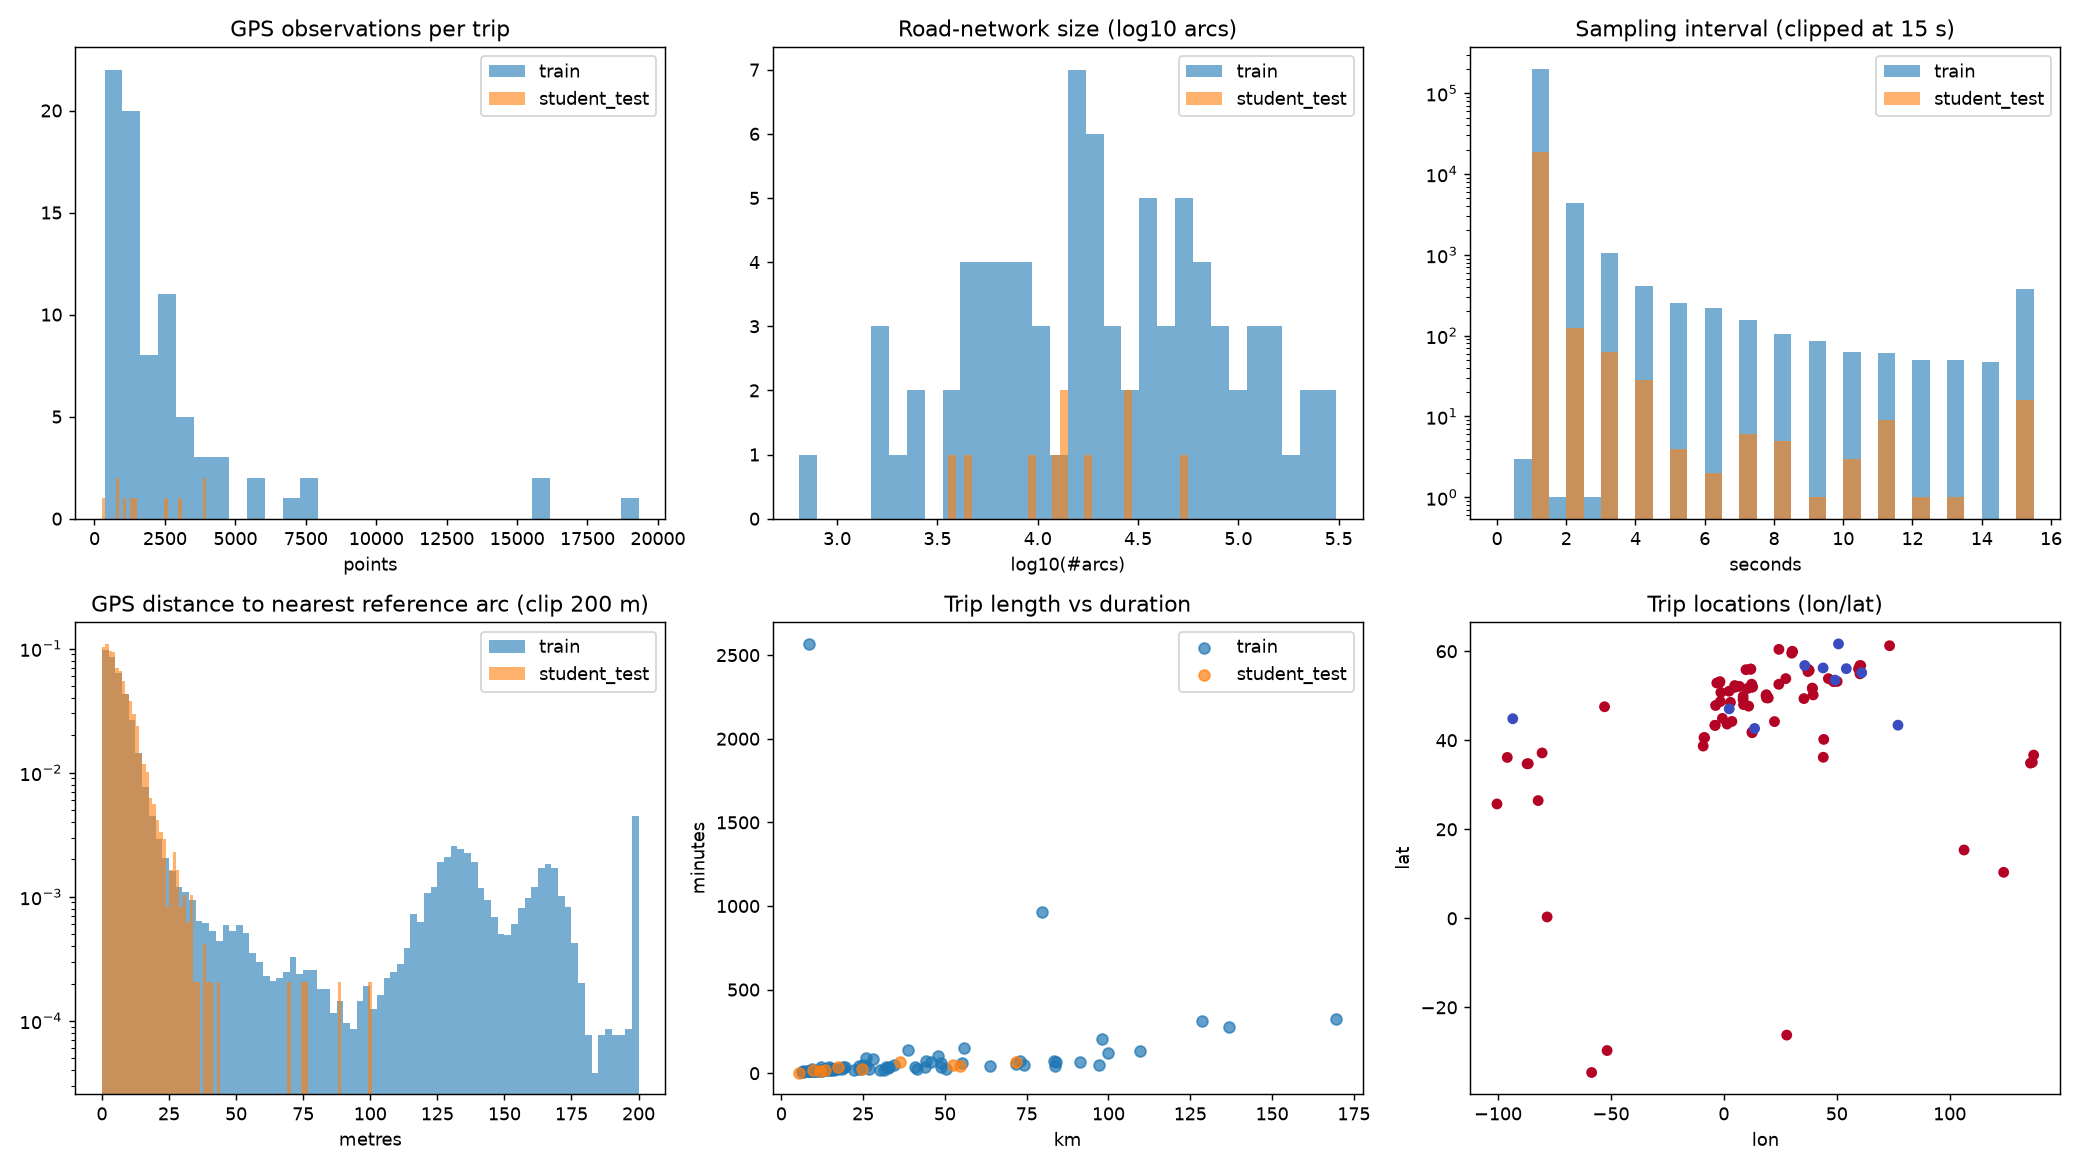
\includegraphics[width=\textwidth]{figures/eda_overview.png}
\caption{EDA overview, train vs.\ student-test: points per trip, network size, sampling interval (log
scale), GPS-to-reference distance (log scale), trip length vs.\ duration, and where the trips are in the
world.}
\end{figure}

\begin{figure}[H]
\centering
\begin{subfigure}{0.48\textwidth}
  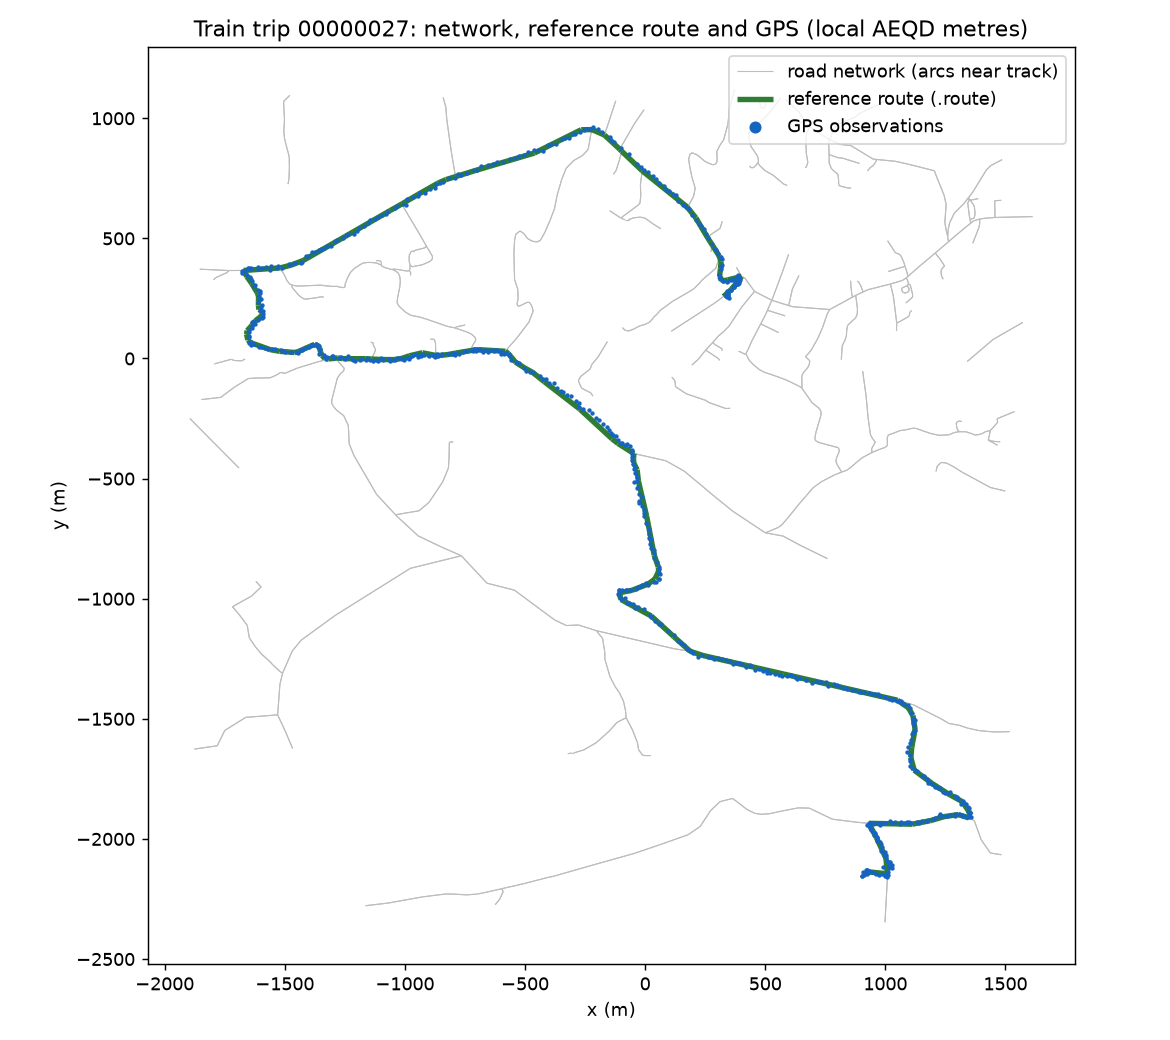
\includegraphics[width=\linewidth]{figures/network_trip27.png}
  \caption{Train trip 00000027: network arcs near the track (grey), reference route (green) and GPS
  (blue), in local metres.}
\end{subfigure}\hfill
\begin{subfigure}{0.48\textwidth}
  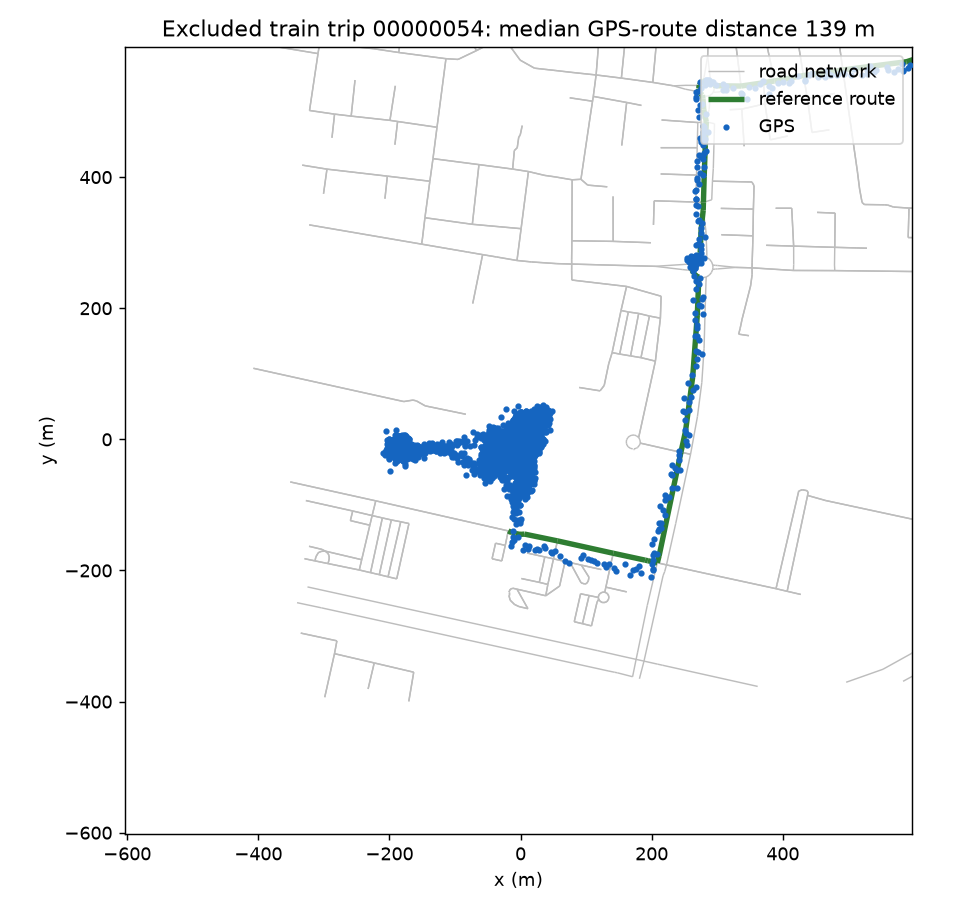
\includegraphics[width=\linewidth]{figures/excluded_trip54.png}
  \caption{Excluded train trip 00000054: a dense GPS cluster that drifts off the mapped network, about
  140\,m from the reference route.}
\end{subfigure}
\caption{Looking at the road networks.}
\end{figure}

\begin{figure}[H]
\centering
\begin{subfigure}{0.56\textwidth}
  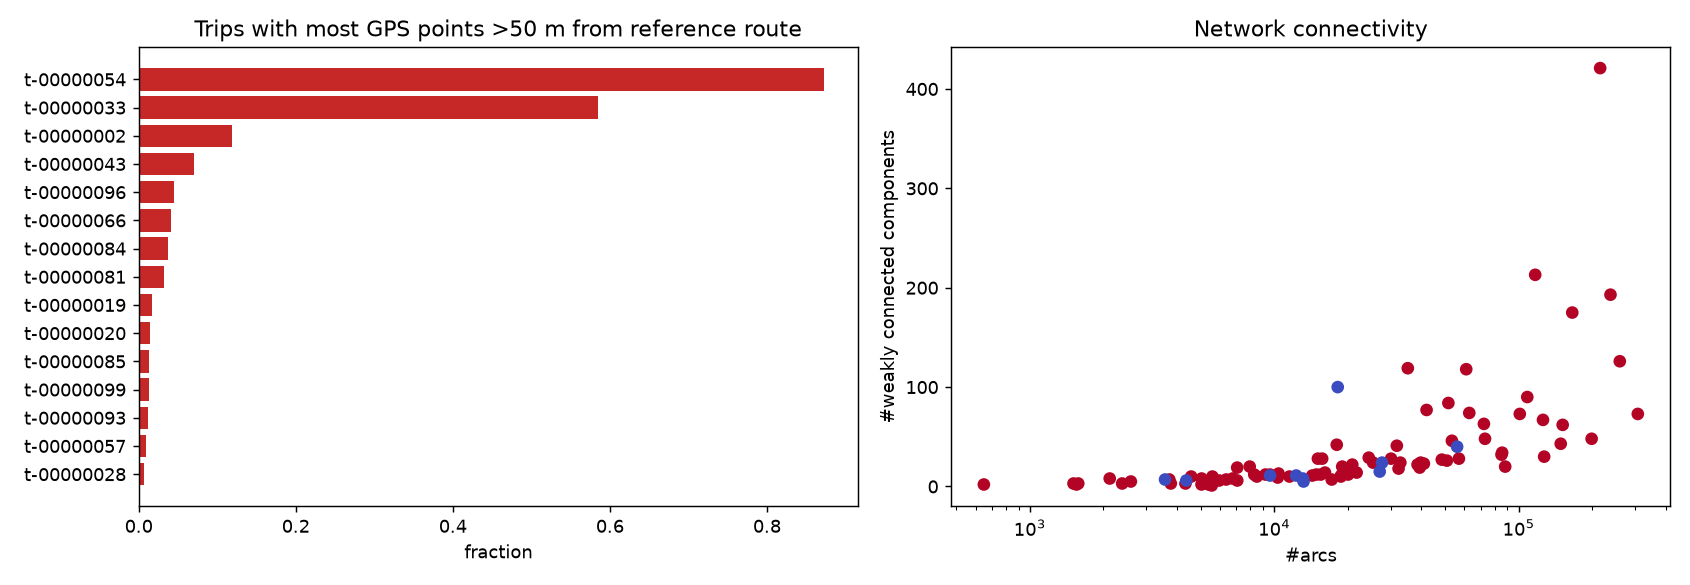
\includegraphics[width=\linewidth]{figures/eda_quality.png}
  \caption{Trips with the most GPS points more than 50\,m from the reference route (left), and network
  connectivity (right).}
\end{subfigure}\hfill
\begin{subfigure}{0.40\textwidth}
  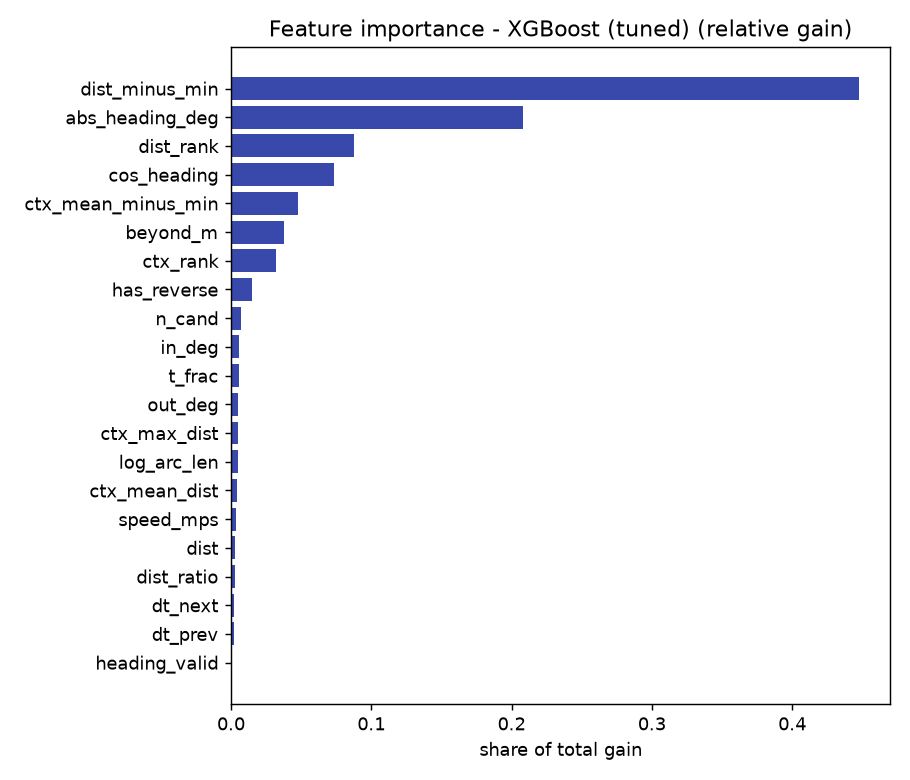
\includegraphics[width=\linewidth]{figures/feature_importance.png}
  \caption{Feature importance of the deployed tuned XGBoost (share of total gain).}
  \label{fig:featimp}
\end{subfigure}
\caption{Data quality and feature importance.}
\end{figure}

\begin{figure}[H]
\centering
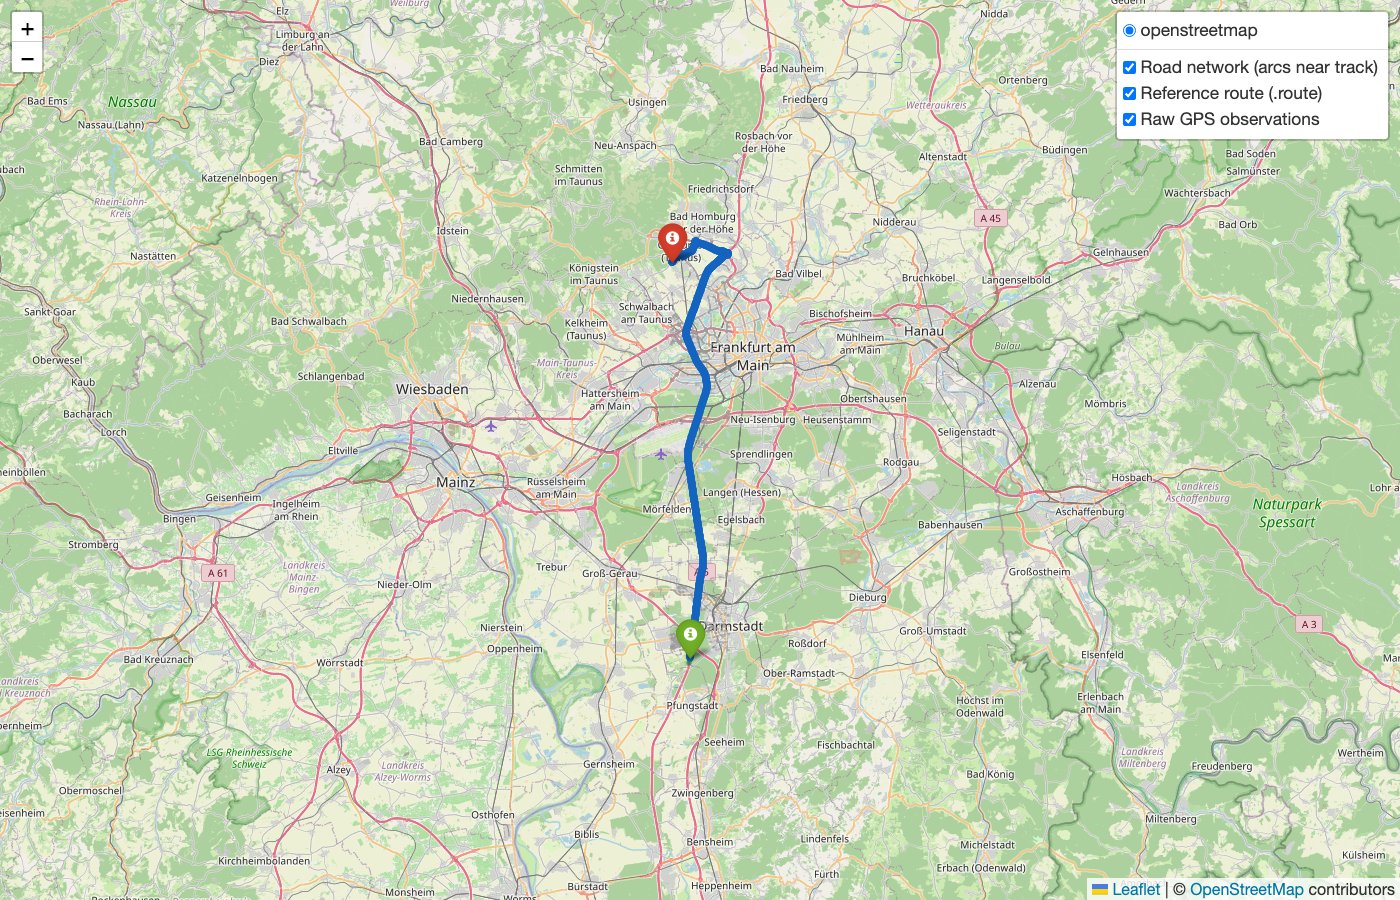
\includegraphics[width=0.85\textwidth]{figures/folium_train01.png}
\caption{Folium map of train trip 00000001: raw GPS (blue), reference route (green), nearby road network
(grey), and start and end markers, with a layer control. The interactive versions are
\code{results/eda/map\_train\_00000001.html} and, for all trip locations,
\code{results/eda/map\_world.html}.}
\end{figure}

% =================================================================== 3
\section{Comparing Models}

\textbf{How we set this up} (\code{scripts/03\_train\_models.py}):
\begin{itemize}
  \item \textbf{Data.} Seven models, one from each of seven algorithm families, all trained on the same 21
        features. That is 1,251,618 labelled candidate rows from the 78 usable training trips.
  \item \textbf{Cross-validation.} 5-fold GroupKFold, grouped by trip, so a trip never ends up in two folds.
        This matters: readings one second apart are almost identical, so a random split would let the
        model see near-copies of its test data.
  \item \textbf{Student-test.} Each model was retrained on all training trips and then scored once on the
        10 student-test trips.
  \item \textbf{How we picked the winner.} The main metric is CV Top-1 accuracy at the observation level:
        how often the highest-scoring candidate is the correct arc. We chose it because that is exactly what
        gets passed on to route reconstruction. Ties go to the model with the lower CV log loss, since the
        HMM uses the probabilities themselves.
  \item \textbf{Candidate-level metrics.} Accuracy, precision, recall, F1 and the confusion matrices use a
        0.5 threshold. We use macro averaging so the smaller ``correct arc'' class counts as much as the
        other one.
  \item \textbf{Route continuity.} The share of consecutive predictions that are either the same arc or
        directly connected arcs.
  \item \textbf{Reproducibility.} The seed is 42 everywhere. Full logs are in
        \code{results/models/experiment\_log.json}.
\end{itemize}

\subsection{Results for all seven models}

\begin{table}[H]
\centering
\scriptsize
\setlength{\tabcolsep}{4pt}
\begin{tabularx}{\textwidth}{@{}l l Y c c c c c c@{}}
\toprule
\textbf{Model} & \textbf{Family} & \textbf{Main settings} & \makecell{\textbf{CV macro}\\\textbf{F1 (sd)}} &
\makecell{\textbf{Top-1}\\\textbf{(test)}} & \makecell{\textbf{Continuity}\\\textbf{(test)}} &
\makecell{\textbf{Macro F1}\\\textbf{(test)}} & \makecell{\textbf{Log loss}\\\textbf{(test)}} &
\makecell{\textbf{Inference}\\\textbf{(test, s)}} \\
\midrule
Logistic Regression & Linear & StandardScaler, L2, $C=1.0$ & 0.9193 (0.012) & 0.8711 & 0.9454 & 0.9159 & 0.1042 & 0.03 \\
Gaussian NB & Generative & var\_smoothing $=10^{-9}$ & 0.7939 (0.011) & 0.8582 & 0.9329 & 0.7900 & 0.8308 & 0.02 \\
KNN & Instance-based & $k=50$, distance-weighted, scaled, 80k-row sample & 0.9159 (0.013) & 0.8678 & 0.9396 & 0.9154 & 0.1182 & 8.35 \\
Random Forest & Bagging & 200 trees, min leaf 5, max\_features sqrt, max\_samples 0.3 & 0.9344 (0.015) & 0.8931 & 0.9525 & 0.9353 & 0.0776 & 0.75 \\
LightGBM & Boosting & 400 trees, lr 0.05, 63 leaves, subsample/colsample 0.8 & 0.9342 (0.015) & 0.8967 & 0.9464 & 0.9374 & 0.0798 & 0.89 \\
\rowcolor{pick}
\textbf{XGBoost (chosen)} & Boosting & 400 trees, lr 0.05, depth 7, subsample/colsample 0.8, hist & \textbf{0.9349} (0.015) & \textbf{0.8984} & \textbf{0.9531} & 0.9349 & \textbf{0.0745} & 0.18 \\
MLP & Neural network & (64, 32) ReLU, Adam, $\alpha=10^{-4}$, batch 512, early stopping, 400k-row sample & 0.9292 (0.014) & 0.8842 & 0.9514 & 0.9290 & 0.0841 & 0.04 \\
\bottomrule
\end{tabularx}
\caption{All seven models. Except for the CV column, every value is on the student-test set. Sources:
\code{results/models/model\_comparison.csv} and \code{cv\_folds.csv}.}
\end{table}

\textbf{CV Top-1} (5-fold mean): LR 0.8785, GNB 0.8619, KNN 0.8701, RF 0.8915, LightGBM 0.8903,
XGBoost 0.8916, MLP 0.8862. Ranked by CV Top-1, with CV log loss as the tie-break, the order is XGBoost, RF,
LightGBM, MLP, LR, KNN, GNB.
\textbf{Training time} on all training trips: LR 2.9\,s, GNB 0.2\,s, KNN 0.01\,s (it does not really train),
RF 106.9\,s, LightGBM 16.0\,s, XGBoost 15.9\,s, MLP 16.9\,s.

\paragraph{Why we chose XGBoost.}
XGBoost and Random Forest are basically tied on CV Top-1 (0.8916 vs.\ 0.8915), so the tie-break and the
practical points decided it:
\begin{itemize}
  \item XGBoost has the best log loss, both in CV (0.0855) and on student-test (0.0745). That means better
        probabilities for the HMM.
  \item Its predictions are about 4 times faster than RF and LightGBM, which matters for a live API.
  \item It trains about 7 times faster than RF.
\end{itemize}
To be honest about it, the fold-to-fold standard deviation of CV Top-1 (about 0.025) is bigger than the gap
between the top three models. All three tree ensembles are equally good classifiers here. Probability quality
and speed are what made the difference.

\subsection{A closer look at each model}

To check for over- and under-fitting, we retrained each model on all training trips, scored it on those same
trips, and compared that with its CV and student-test scores (\code{results/models/train\_vs\_cv\_vs\_test.csv}).

\begin{table}[H]
\centering
\small
\begin{tabular}{@{}lccccccc@{}}
\toprule
\textbf{Model} & \makecell{\textbf{Train}\\\textbf{Top-1}} & \makecell{\textbf{CV}\\\textbf{Top-1}} & \makecell{\textbf{Test}\\\textbf{Top-1}} &
\makecell{\textbf{Train}\\\textbf{$-$ CV}} & \makecell{\textbf{Train}\\\textbf{log loss}} & \makecell{\textbf{CV}\\\textbf{log loss}} & \makecell{\textbf{Test}\\\textbf{log loss}} \\
\midrule
Logistic Regression & 0.8788 & 0.8785 & 0.8711 & 0.0002 & 0.1109 & 0.1120 & 0.1042 \\
Gaussian NB & 0.8619 & 0.8619 & 0.8582 & 0.0000 & 0.8796 & 0.8722 & 0.8308 \\
KNN & 0.8874 & 0.8701 & 0.8678 & 0.0173 & 0.1048 & 0.1375 & 0.1182 \\
Random Forest & 0.9228 & 0.8915 & 0.8931 & 0.0313 & 0.0586 & 0.0862 & 0.0776 \\
LightGBM & 0.9275 & 0.8903 & 0.8967 & 0.0372 & 0.0573 & 0.0897 & 0.0798 \\
\rowcolor{pick}
XGBoost & 0.9267 & 0.8916 & 0.8984 & 0.0351 & 0.0581 & 0.0855 & 0.0745 \\
MLP & 0.9021 & 0.8862 & 0.8842 & 0.0159 & 0.0771 & 0.0929 & 0.0841 \\
\bottomrule
\end{tabular}
\caption{Training vs.\ CV vs.\ student-test scores.}
\end{table}

\subsubsection*{Model 1 -- Logistic Regression (linear)}
\textbf{Why it fits the problem.} It is a strong baseline that is easy to interpret, and it gives
reasonable-looking probabilities, which the HMM needs. Several of the key signals point in one direction: a
smaller relative distance and a smaller heading difference should both raise the probability.\\
\textbf{Strengths and limits.} It is fast (2.9\,s to train, 0.03\,s to predict) and the most stable across
folds (CV F1 sd 0.012). But it can only draw a straight-line boundary through the scaled features, so it
misses interactions. For example, heading only matters when the point is close to the arc and the car is
moving fast enough for the heading to mean something.\\
\textbf{Settings.} $C=1.0$ (inverse L2 strength), L2 penalty, lbfgs solver, max\_iter 2000. Features are
scaled with a StandardScaler fitted on the training folds only.\\
\textbf{Objective.} Binary cross-entropy (log loss) with L2 regularisation.\\
\textbf{Student-test.} Accuracy 0.9600, macro F1 0.9159, precision 0.9111, recall 0.9209, log loss 0.1042,
Top-1 0.8711, continuity 0.9454.\\
\textbf{Fit.} \emph{Under-fitting (high bias).} Train Top-1 (0.8788) and CV (0.8785) are almost the same,
and both sit about 1.3 points below the tree models. More data would not close that gap; only a more
flexible model would.

\subsubsection*{Model 2 -- Gaussian Naive Bayes (probabilistic, generative)}
\textbf{Why it fits the problem.} It is the simplest probabilistic model. It fits a Gaussian to each feature
for each class and gives $P(\text{correct arc}\mid\text{features})$ directly. We used it as a lower bound,
and to see how well the features separate the classes on their own.\\
\textbf{Strengths and limits.} It is the fastest to train (0.2\,s). But it assumes the features are
independent and normally distributed, and ours are neither. \code{dist}, \code{dist\_rank},
\code{dist\_minus\_min} and \code{dist\_ratio} all describe distance, and they are heavily skewed. So Naive
Bayes counts the same evidence several times and becomes over-confident.\\
\textbf{Settings.} var\_smoothing $=10^{-9}$ (the default). There is nothing else to set.\\
\textbf{Objective.} Maximum-likelihood estimates of each class's feature means and variances.\\
\textbf{Student-test.} Accuracy 0.8674, macro F1 0.7900, precision 0.7493, recall 0.9055, log loss 0.8308
(about 8 times worse than the rest), Top-1 0.8582, continuity 0.9329.\\
\textbf{Fit.} \emph{Under-fitting, because the model's assumptions are wrong for this data.} Train, CV and
test agree (0.862 / 0.862 / 0.858), but the log loss is very high. High recall with low precision tells us it
calls too many candidates positive. Its Top-1 is still not bad, because within one point it usually ranks
the candidates in the right order even when the probabilities themselves are off.

\subsubsection*{Model 3 -- K-Nearest Neighbours (instance-based)}
\textbf{Why it fits the problem.} Candidates with similar geometry (distance, heading, context) should have
the same label. A similarity-based classifier follows that idea directly, without assuming any
distribution.\\
\textbf{Strengths and limits.} There is no real training, and the decision boundary can take any shape. On
the other hand it needs scaled features and is by far the slowest to predict: 8.35\,s for the student-test
set, about 50 times slower than XGBoost. In 21 dimensions the ``nearest'' neighbours are also less
meaningful. We could only fit it on an 80,000-row sample to keep prediction time reasonable.\\
\textbf{Settings.} $k=50$, distance-weighted votes, Euclidean distance on scaled features, 80k training rows
(sampled as whole observations).\\
\textbf{Objective.} None; KNN just stores the data. Each prediction is the distance-weighted vote of the 50
closest training candidates.\\
\textbf{Student-test.} Accuracy 0.9602, macro F1 0.9154, precision 0.9144, recall 0.9164, log loss 0.1182,
Top-1 0.8678, continuity 0.9396.\\
\textbf{Fit.} \emph{Mild over-fitting.} Train Top-1 0.8874 vs.\ CV 0.8701 (a gap of 0.017), and train log
loss 0.105 vs.\ CV 0.138. With distance weighting, a training point effectively votes for itself. CV and test
agree (0.870 vs.\ 0.868), so it generalises consistently, but the small sample holds it back.

\subsubsection*{Model 4 -- Random Forest (bagging ensemble)}
\textbf{Why it fits the problem.} Trees naturally learn rules like ``if this is the closest candidate
\emph{and} the heading agrees, it is probably correct''. Averaging many different trees also reduces the
effect of noisy labels.\\
\textbf{Strengths and limits.} Second-best CV Top-1 (0.8915) and a good log loss (0.0776). It is also the
most expensive model we trained: 106.9\,s to train and 0.75\,s to predict. Its probabilities are just vote
shares, so they can be less sharp than boosting's.\\
\textbf{Settings.} 200 trees, min\_samples\_leaf 5, max\_features ``sqrt'', max\_samples 0.3 (each tree sees a
30\% bootstrap sample, to save time), no depth limit.\\
\textbf{Objective.} Each tree greedily minimises Gini impurity, and the forest averages the trees' class
probabilities.\\
\textbf{Student-test.} Accuracy 0.9699, macro F1 0.9353, precision 0.9395, recall 0.9313, log loss 0.0776,
Top-1 0.8931, continuity 0.9525.\\
\textbf{Fit.} \emph{Moderate over-fitting.} Train Top-1 0.9228 vs.\ CV 0.8915 (a gap of 0.031), and train
log loss 0.059 vs.\ CV 0.086. That is expected with unlimited depth. Since CV and test agree (0.8915 vs.\
0.8931), the over-fitting does not hurt on new trips; it is mostly the trees memorising label noise.

\subsubsection*{Model 5 -- LightGBM (gradient boosting)}
\textbf{Why it fits the problem.} Gradient-boosted trees are the standard choice for table-shaped data with
non-linear features on different scales. Each new tree corrects the mistakes of the earlier ones, such as
the hard cases at junctions.\\
\textbf{Strengths and limits.} Best student-test macro F1 (0.9374) and fast training (16.0\,s). Growing trees
leaf by leaf with 63 leaves can over-fit, though, and in our setup it predicted more slowly than XGBoost
(0.89\,s).\\
\textbf{Settings.} 400 trees, learning rate 0.05, 63 leaves, subsample 0.8 (every iteration),
colsample\_bytree 0.8.\\
\textbf{Objective.} Binary log loss, minimised with second-order gradient boosting.\\
\textbf{Student-test.} Accuracy 0.9708, macro F1 0.9374, precision 0.9395, recall 0.9354, log loss 0.0798,
Top-1 0.8967, continuity 0.9464.\\
\textbf{Fit.} \emph{Moderate over-fitting.} Train Top-1 0.9275 vs.\ CV 0.8903, the largest gap of any model
(0.037). CV and test are still consistent (0.890 vs.\ 0.897), so it generalises, but it is slightly behind
XGBoost on CV Top-1 and log loss.

\subsubsection*{Model 6 -- XGBoost (gradient boosting) -- chosen}
\textbf{Why it fits the problem.} Everything said about LightGBM applies here too. On top of that, XGBoost
grows trees level by level and applies L2 regularisation to the leaf weights. That gave the best-calibrated
probabilities (lowest log loss), which matters because the HMM multiplies these probabilities along the
whole sequence.\\
\textbf{Strengths and limits.} Best CV Top-1 (0.8916), best CV and test log loss, and fast predictions
(0.18\,s for 140k candidates, about 0.009\,ms per point). It is harder to interpret than logistic regression.
The feature importance (Fig.~\ref{fig:featimp}) shows it relies mainly on relative distance and heading,
which matches how we think about the task. It still judges each point on its own; the HMM fixes that
(Section~\ref{sec:hmm}).\\
\textbf{Starting settings.} 400 trees, learning rate 0.05, max depth 7, subsample 0.8, colsample\_bytree 0.8,
hist tree method, min\_child\_weight 1, reg\_lambda 1. The tuned values are in Section~\ref{sec:bo}.\\
\textbf{Objective.} \code{binary:logistic} (log loss) with L2 regularisation on the leaf weights.\\
\textbf{Student-test.} Accuracy 0.9697, macro F1 0.9349, precision 0.9388, recall 0.9310, log loss 0.0745,
Top-1 0.8984, continuity 0.9531, route F1 (classifier only) 0.9011.\\
\textbf{Fit.} \emph{Moderate over-fitting.} Train Top-1 0.9267 vs.\ CV 0.8916 (a gap of 0.035), and train
log loss 0.058 vs.\ CV 0.086. On student-test it scores 0.8984, at least as well as in CV, so it holds up on
trips and cities it has never seen. Much of the remaining gap between training and CV is label noise near
junctions, which no model can learn honestly.

\subsubsection*{Model 7 -- Multi-layer Perceptron (neural network)}
\textbf{Why it fits the problem.} A small neural network can learn smooth non-linear combinations of the
geometric features, and its sigmoid output gives a probability.\\
\textbf{Strengths and limits.} Fast predictions (0.04\,s) and good continuity (0.951). It needs scaled
features and careful regularisation, we had to train it on a 400k-row sample to save time, and it still
falls behind the tree models on this kind of table data (Top-1 0.884).\\
\textbf{Settings.} Hidden layers (64, 32), ReLU, Adam with learning rate $10^{-3}$, L2 $\alpha=10^{-4}$,
batch 512, max\_iter 60, early stopping (10\% held out, patience 6), StandardScaler.\\
\textbf{Objective.} Binary cross-entropy plus an L2 penalty, minimised with Adam.\\
\textbf{Student-test.} Accuracy 0.9673, macro F1 0.9290, precision 0.9373, recall 0.9211, log loss 0.0841,
Top-1 0.8842, continuity 0.9514.\\
\textbf{Fit.} \emph{Slight over-fitting, kept in check by early stopping.} Train Top-1 0.9021 vs.\ CV 0.8862
(a gap of 0.016). The training loss keeps going down, but accuracy on the 10\% hold-out levels off at about
0.970 after roughly 25 epochs. Early stopping (6 epochs with no improvement) ended training at epoch 40,
before the network could keep fitting noise (Fig.~\ref{fig:mlp}). It is the only model with a history per
epoch, so it is the only one with a training curve.

\subsection{Plots}

\begin{figure}[H]
\centering
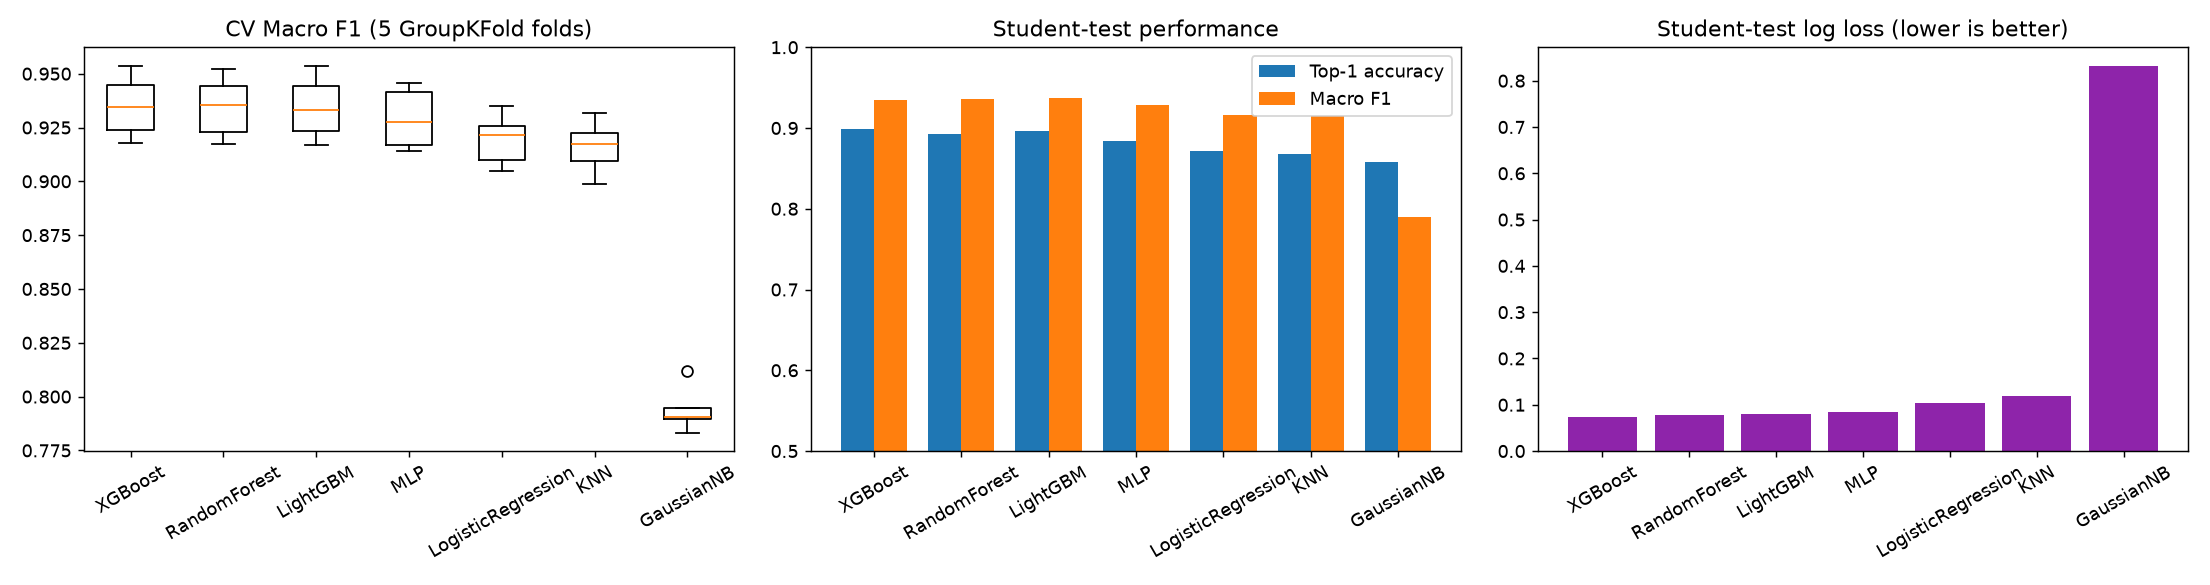
\includegraphics[width=\textwidth]{figures/model_comparison.png}
\caption{Left: CV macro F1 across the 5 GroupKFold folds for each model. Middle: student-test Top-1 and
macro F1. Right: student-test log loss.}
\end{figure}

\begin{figure}[H]
\centering
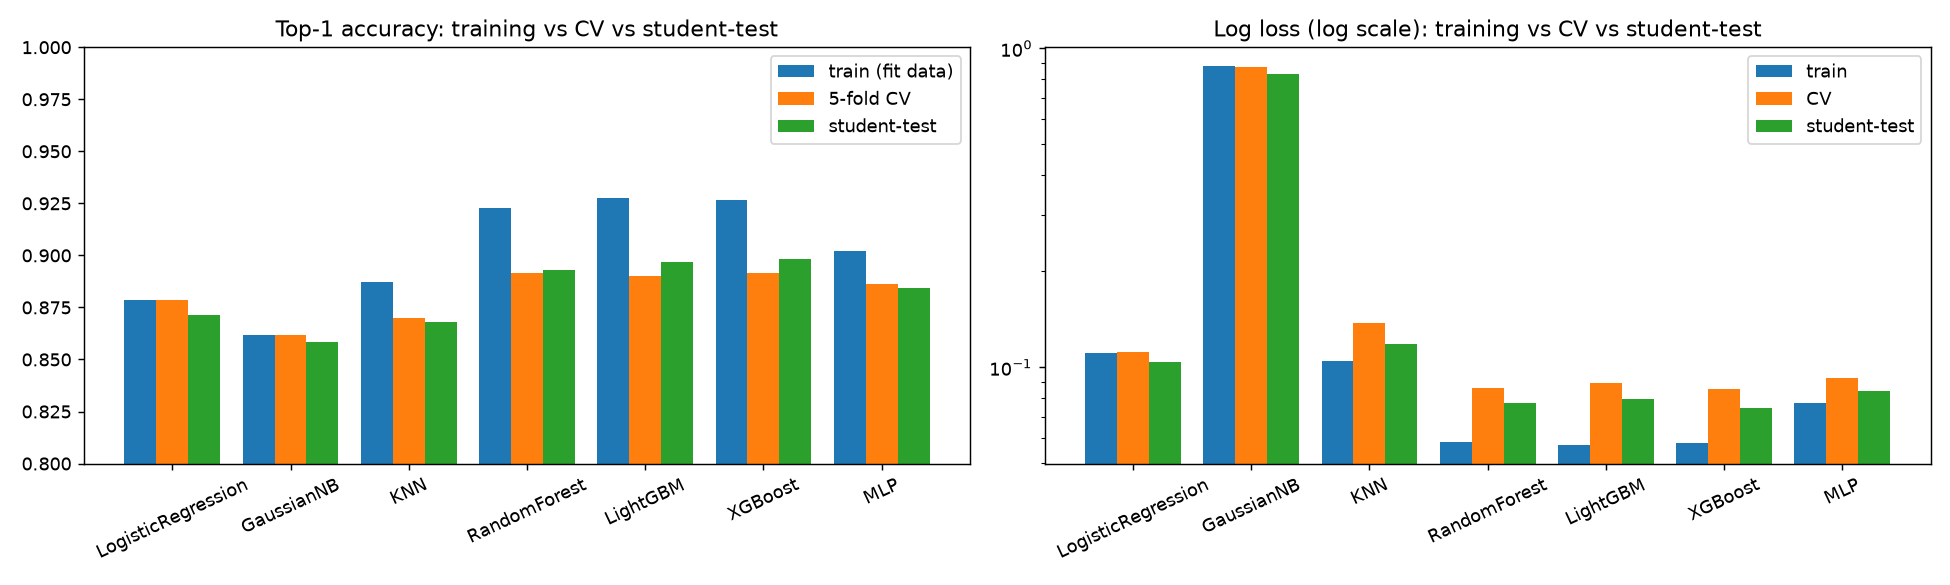
\includegraphics[width=\textwidth]{figures/train_cv_test.png}
\caption{Evidence of over- and under-fitting: Top-1 and log loss on training data, in CV, and on
student-test.}
\end{figure}

\begin{figure}[H]
\centering
\begin{subfigure}{0.52\textwidth}
  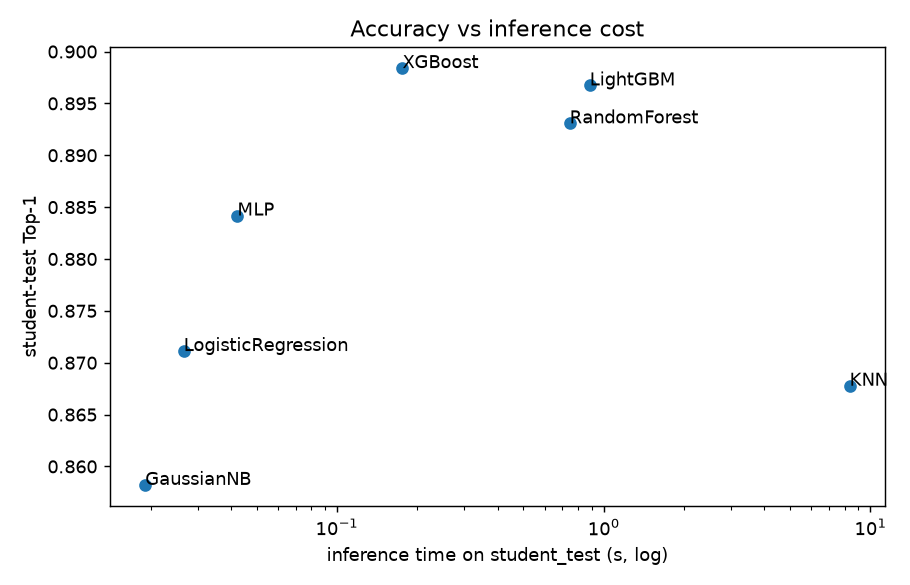
\includegraphics[width=\linewidth]{figures/accuracy_vs_time.png}
  \caption{Student-test Top-1 vs.\ prediction time (log scale). XGBoost gives the best balance of accuracy
  and cost.}
\end{subfigure}\hfill
\begin{subfigure}{0.44\textwidth}
  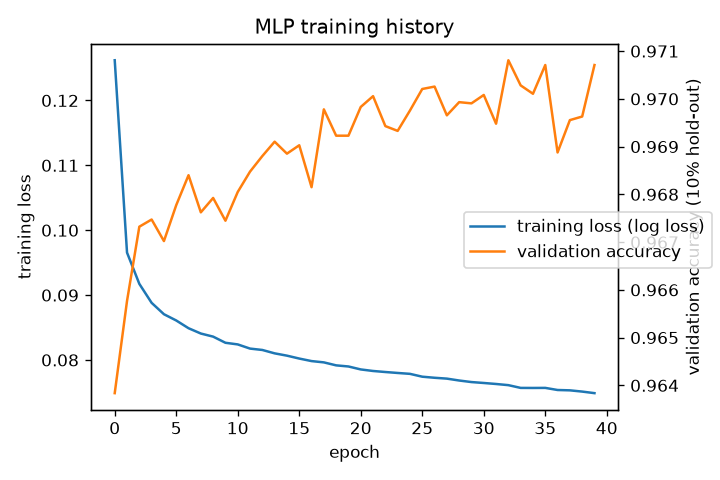
\includegraphics[width=\linewidth]{figures/mlp_history.png}
  \caption{MLP training loss and hold-out accuracy per epoch.}
  \label{fig:mlp}
\end{subfigure}
\caption{Cost of each model, and how the MLP trained.}
\end{figure}

\begin{figure}[H]
\centering
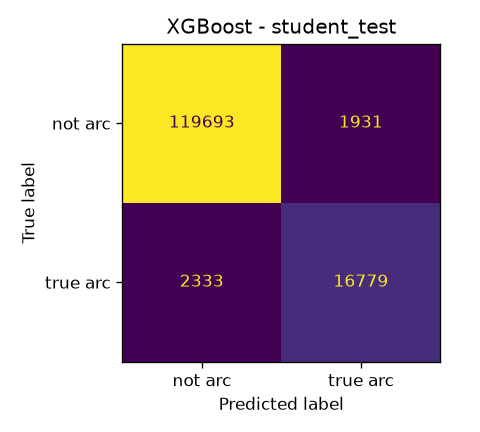
\includegraphics[width=0.24\textwidth]{figures/cm_xgboost.png}\hfill
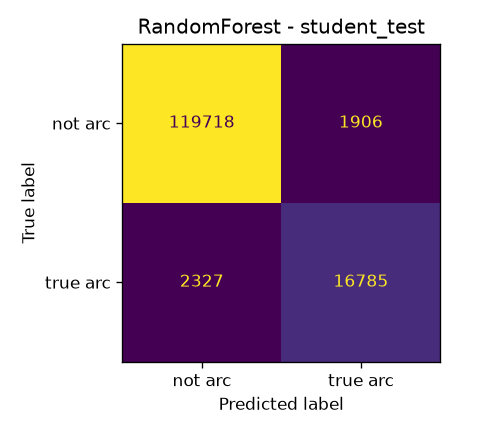
\includegraphics[width=0.24\textwidth]{figures/cm_rf.png}\hfill
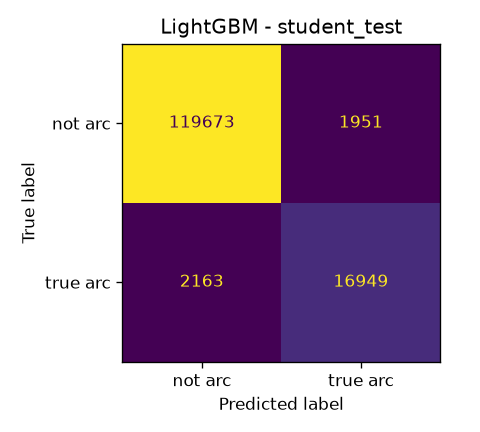
\includegraphics[width=0.24\textwidth]{figures/cm_lgbm.png}\hfill
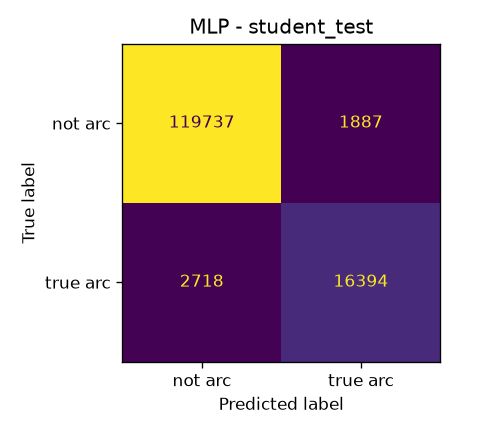
\includegraphics[width=0.24\textwidth]{figures/cm_mlp.png}\\[0.4em]
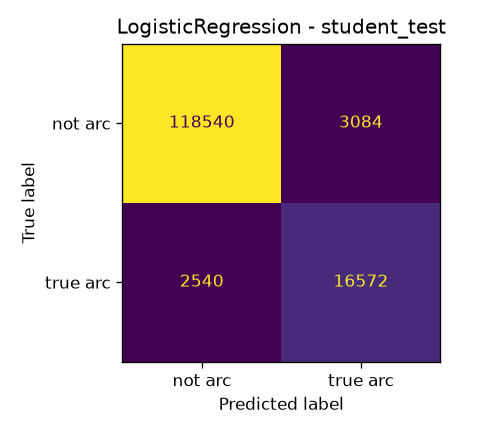
\includegraphics[width=0.24\textwidth]{figures/cm_lr.png}\hspace{0.8em}
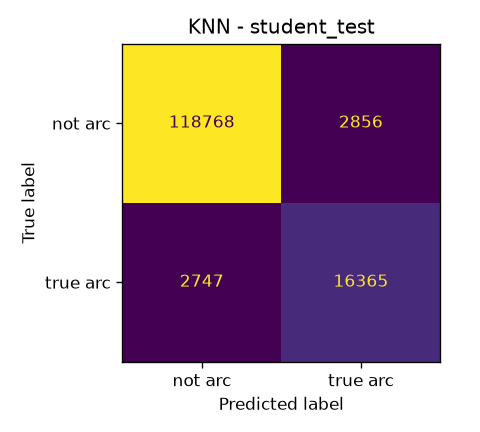
\includegraphics[width=0.24\textwidth]{figures/cm_knn.png}\hspace{0.8em}
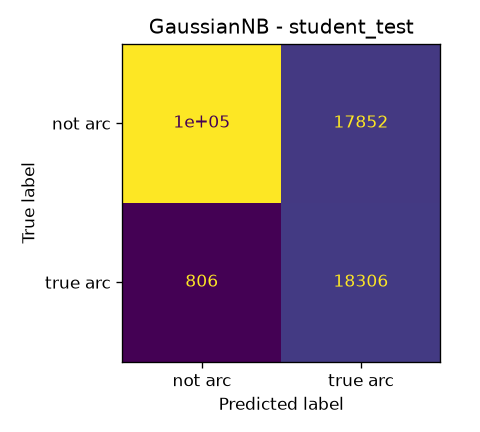
\includegraphics[width=0.24\textwidth]{figures/cm_gnb.png}
\caption{Student-test confusion matrices (threshold 0.5) for all seven models.}
\end{figure}

% =================================================================== 4
\section{Bayesian Hyperparameter Tuning of XGBoost}
\label{sec:bo}

The code is in \code{scripts/04\_bayes\_opt.py}, and the outputs are in \code{results/bayes\_opt/}. We used
only the training trips. The evaluator data played no part in the search space, the objective or any
threshold.

\begin{enumerate}
  \item \textbf{What we searched over:} n\_estimators, learning\_rate, max\_depth, min\_child\_weight,
        subsample, colsample\_bytree and reg\_lambda.
  \item \textbf{Ranges:}
  \begin{itemize}
    \item n\_estimators: 100--800, in steps of 50
    \item learning\_rate: 0.01--0.2, log-uniform
    \item max\_depth: 3--12, integer
    \item min\_child\_weight: 0.5--20, log-uniform
    \item subsample: 0.5--1.0
    \item colsample\_bytree: 0.4--1.0
    \item reg\_lambda: 0.001--10, log-uniform
  \end{itemize}
  The ranges are centred on the untuned settings and wide enough to reach both shallow, heavily regularised
  models and deep ones. Parameters whose effect is multiplicative use a log scale.
  \item \textbf{Objective.} Maximise the mean observation-level Top-1 accuracy over a 3-fold GroupKFold (by
        trip) on the 78 training trips. This is the same metric we used to pick the model. We used three folds
        instead of five so each trial took about 50\,s.
  \item \textbf{Trials.} 30, with Optuna's TPE sampler (seed 42). The whole search took 1,603\,s (26.7
        minutes) on 8 CPU cores. Trial scores ranged from 0.8838 to 0.8905.
  \item \textbf{Best values:} n\_estimators 600, learning\_rate 0.0102, max\_depth 10, min\_child\_weight 3.73,
        subsample 0.587, colsample\_bytree 0.882, reg\_lambda 0.745. In other words: a lower learning rate
        with more and deeper trees, balanced by stronger row subsampling and a larger minimum child weight.
  \item \textbf{Did tuning help?} Barely. 3-fold CV Top-1 went up by 0.0004 (0.8902 to 0.8905), 5-fold CV
        macro F1 by 0.0003, and student-test log loss improved from 0.0745 to 0.0739. Student-test Top-1
        actually dropped by 0.0015. All of these changes are well inside the fold-to-fold spread (CV Top-1 sd
        about 0.025), and the tuned model predicts 2.7 times more slowly. We still deployed the tuned model,
        because our rule, fixed in advance, was ``take the higher CV objective'', and we did not let the
        student-test numbers change that choice. Our reading is that the default settings were already close to
        the best possible, and the limit comes from the features and from label noise near junctions, not from
        model capacity.
\end{enumerate}

\begin{table}[H]
\centering
\small
\begin{tabular}{@{}lccccccc@{}}
\toprule
\textbf{Version} & \makecell{\textbf{CV macro F1}\\\textbf{(5-fold)}} & \makecell{\textbf{CV Top-1}\\\textbf{(3-fold)}} &
\makecell{\textbf{Test}\\\textbf{Top-1}} & \makecell{\textbf{Test}\\\textbf{macro F1}} & \makecell{\textbf{Test}\\\textbf{log loss}} &
\makecell{\textbf{Train}\\\textbf{time (s)}} & \makecell{\textbf{Inference}\\\textbf{time (s)}} \\
\midrule
Untuned XGBoost & 0.9349 & 0.8902 & 0.8984 & 0.9349 & 0.0745 & 16.5 & 0.18 \\
\rowcolor{pick}
Tuned XGBoost (deployed) & 0.9352 & 0.8905 & 0.8969 & 0.9382 & 0.0739 & 33.7 & 0.49 \\
\bottomrule
\end{tabular}
\caption{Untuned vs.\ tuned XGBoost.}
\end{table}

\begin{figure}[H]
\centering
\begin{subfigure}{0.52\textwidth}
  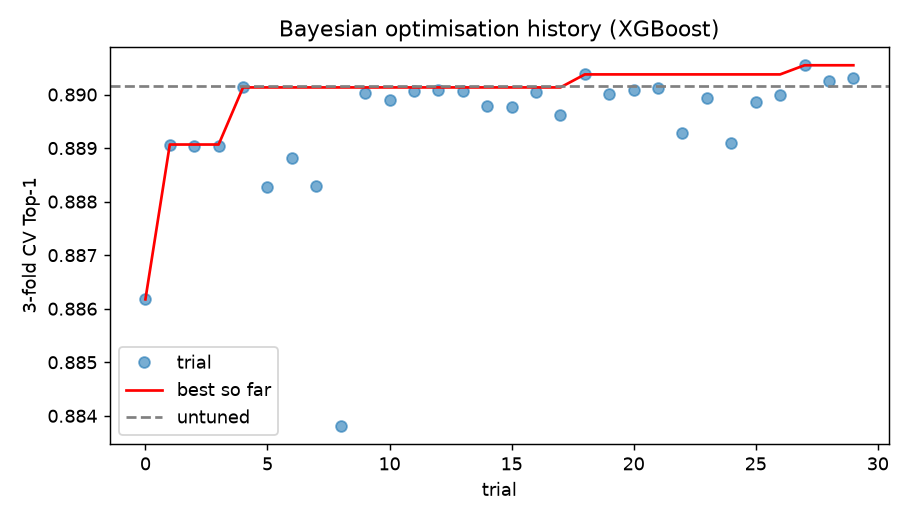
\includegraphics[width=\linewidth]{figures/bo_history.png}
  \caption{Optimisation history: each trial's 3-fold CV Top-1, the best so far (red), and the untuned
  baseline (dashed).}
\end{subfigure}\hfill
\begin{subfigure}{0.44\textwidth}
  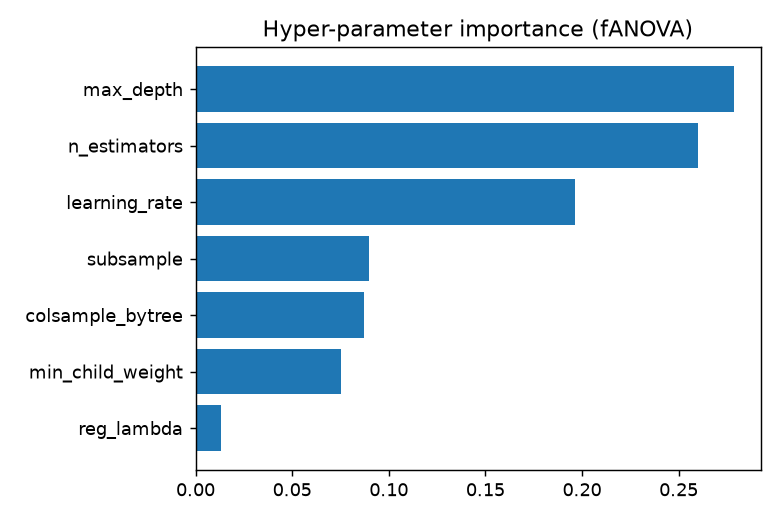
\includegraphics[width=\linewidth]{figures/bo_importance.png}
  \caption{Hyperparameter importance (fANOVA) over the 30 trials.}
\end{subfigure}
\caption{Bayesian optimisation.}
\end{figure}

% =================================================================== 5
\section{Rebuilding the Route with an HMM and Viterbi}
\label{sec:hmm}

The code is in \code{src/pathsnap/hmm.py}, \code{src/pathsnap/pipeline.py} and \code{scripts/05\_hmm.py},
and the outputs are in \code{results/hmm/}.

The classifier looks at each GPS point on its own. That leaves room for answers that cannot happen in real
life, such as jumping to a parallel road for one second and then jumping back. The HMM looks at the whole
trip and asks which sequence of arcs a car could actually have driven.

\paragraph{1. Hidden states.}
At step $i$, the hidden states are the candidate arcs of GPS point $i$ (at most 10). Each state keeps its arc
id, its two endpoints, and how far along the arc the point projects (\code{along\_m}). So every state still
corresponds to a specific candidate, and Viterbi returns one arc id per point.

\paragraph{2. Emission probabilities.}
We take the tuned XGBoost probability, normalise it over that point's candidates, and sharpen it with a
weight $w$:
\[
\log E_i(c) \;=\; w \cdot \log\!\left(\frac{p_i(c)}{\sum_{c'} p_i(c')}\right), \qquad w = 2.0\ \text{(tuned)}
\]

\paragraph{3. Transition probabilities.}
We follow Newson and Krumm. For candidate $a$ at step $i$ and candidate $b$ at step $i+1$:
\begin{itemize}
  \item $d_\text{route}$ is the distance you would actually drive from the point's position on $a$ to its
        position on $b$. If $a$ and $b$ are the same arc, it is just the distance along that arc, with up to
        15\,m of backward jitter allowed. Otherwise it is the rest of $a$, plus the shortest directed path from
        the end of $a$ to the start of $b$ (a bounded Dijkstra search), plus the offset along $b$.
  \item $d_\text{gc}$ is the straight-line distance between the two GPS readings.
\end{itemize}
\[
\log T(a,b) \;=\; -\,\frac{\lvert d_\text{route} - d_\text{gc}\rvert}{\beta}, \qquad \beta = 2.0\,\text{m (tuned)}
\]
If $b$ cannot be reached from $a$ within $2\,d_\text{gc} + 150$\,m, the transition gets $-\infty$.
In plain terms, this prefers moves where the distance driven matches how far the GPS actually moved. It
also rules out moves that are impossible, like going the wrong way down a one-way arc or jumping between
roads that do not connect.

\paragraph{Viterbi.}
We work in log space and keep back-pointers:
\[
\delta_1(c) = \log E_1(c), \qquad
\delta_{i+1}(b) = \log E_{i+1}(b) + \max_a\big[\delta_i(a) + \log T(a,b)\big], \qquad
\psi_{i+1}(b) = \arg\max_a\big[\cdots\big]
\]
We take the best final state and follow $\psi$ back to the start. Scores are re-normalised at every step so
the numbers do not underflow.

\paragraph{4. Points with no candidates, and big GPS gaps.}
\begin{itemize}
  \item Points with no candidate within 60\,m are skipped and returned as unmatched ($-1$).
  \item If two readings are more than 60\,s apart or more than 1.5\,km apart, we cut the chain: we finish
        the current segment, trace it back, and start a new chain from the emissions alone. This stops the
        decoder from forcing a path across something like the 153,064\,s gap in training trip 00000090.
  \item On student-test this happened 2 times in trip 00000000, once in 00000056, once in 00000065, and
        nowhere else.
\end{itemize}

\paragraph{5. When consecutive arcs do not connect.}
If no candidate at step $i+1$ can be reached from any candidate at step $i$, every transition is $-\infty$.
We then cut the chain the same way instead of producing an impossible jump. After decoding,
\code{fill\_route} inserts the shortest directed path between consecutive matched arcs that are not directly
connected. This happens, for example, when the car crosses a short arc between two readings one second
apart. Gaps that cannot be bridged within 3\,km are left open. There were 3 of these on student-test (2 in
trip 00000000 and 1 in 00000056), all at the chain breaks caused by large GPS gaps.

\paragraph{6. Did the HMM help?}
Yes, on every student-test trip (see the table and Fig.~\ref{fig:hmmtrip}):
\begin{itemize}
  \item Pooled Top-1 accuracy went from 0.8970 to 0.9361 (+3.9 points).
  \item Point-by-point continuity went from 0.953 to 0.979.
  \item Route F1 went from 0.899 to 0.928 with the HMM, and to 0.967 after gap filling, with continuity
        0.999.
\end{itemize}

\paragraph{Tuning the decoder without leakage.}
We picked $\beta$ and $w$ with a grid search over $\beta \in \{1, 2, 3, 6, 12, 25, 50\}$\,m and
$w \in \{0.25, 0.5, 1, 2\}$. The search ran on 16 training trips using out-of-fold XGBoost probabilities, so
each trip's probabilities came from a model that had never seen that trip. The best setting was $\beta = 2$,
$w = 2$, with Top-1 0.9236 compared with 0.8887 for the classifier alone on the same trips. The results are
fairly flat for small $\beta$: every setting with $\beta \le 6$\,m and $w \ge 0.5$ scores between 0.921 and
0.924. A large $\beta$ combined with a large $w$ ($\beta = 50$, $w = 2$) drops to 0.910, because the decoder
then trusts the classifier too much and the road connections too little. We did not use the student-test
trips for this tuning.

\begin{table}[H]
\centering
\small
\begin{tabular}{@{}lcccccc@{}}
\toprule
\textbf{Method (student-test, 10 trips)} & \makecell{\textbf{Top-1}\\\textbf{(pooled)}} & \makecell{\textbf{Top-1}\\\textbf{(trip mean)}} &
\textbf{Continuity} & \makecell{\textbf{Route}\\\textbf{precision}} & \makecell{\textbf{Route}\\\textbf{recall}} & \makecell{\textbf{Route}\\\textbf{F1}} \\
\midrule
Classifier only (best per point) & 0.8970 & 0.9091 & 0.9532 & 0.9091 & 0.8937 & 0.8991 \\
Classifier + HMM/Viterbi & 0.9361 & 0.9434 & 0.9785 & 0.9587 & 0.9025 & 0.9282 \\
\rowcolor{pick}
Classifier + HMM + gap filling (deployed) & 0.9361 & 0.9434 & 0.9990 & 0.9448 & 0.9920 & 0.9673 \\
\bottomrule
\end{tabular}
\caption{What the HMM and gap filling add.}
\end{table}

\begin{table}[H]
\centering
\small
\begin{tabular}{@{}lrccccc@{}}
\toprule
\textbf{Trip} & \textbf{Points} & \makecell{\textbf{Top-1}\\\textbf{classifier}} & \makecell{\textbf{Top-1}\\\textbf{HMM}} &
\makecell{\textbf{Route F1}\\\textbf{classifier}} & \makecell{\textbf{Route F1}\\\textbf{HMM}} & \makecell{\textbf{Route F1}\\\textbf{HMM + fill}} \\
\midrule
00000000 & 2,503 & 0.9529 & 0.9656 & 0.9169 & 0.9428 & 0.9368 \\
00000007 & 1,354 & 0.9276 & 0.9542 & 0.9837 & 0.9878 & 0.9878 \\
00000009 & 1,049 & 0.8875 & 0.9190 & 0.8676 & 0.8845 & 0.9580 \\
00000040 & 2,995 & 0.9549 & 0.9743 & 0.9391 & 0.9720 & 0.9952 \\
00000052 & 262 & 0.9733 & 1.0000 & 0.8814 & 0.9266 & 0.9894 \\
00000056 & 3,958 & 0.9166 & 0.9575 & 0.9108 & 0.9312 & 0.9607 \\
00000065 & 768 & 0.8711 & 0.8919 & 0.8966 & 0.9399 & 0.9797 \\
00000076 & 1,486 & 0.9253 & 0.9704 & 0.8698 & 0.9129 & 0.9451 \\
00000077 & 3,911 & 0.7760 & 0.8530 & 0.8769 & 0.9297 & 0.9420 \\
00000091 & 874 & 0.9062 & 0.9485 & 0.8485 & 0.8544 & 0.9788 \\
\bottomrule
\end{tabular}
\caption{Per-trip results on student-test.}
\end{table}

\paragraph{Where the HMM helped most.}
Trip 00000077 gained 7.7 points of Top-1. It is a city trip where the classifier on its own keeps flipping
between neighbouring arcs (its continuity is 0.959). Requiring arcs to connect removes those one-off flips,
and continuity rises to 0.993 after decoding.

\paragraph{Where it did not help, or made things slightly worse.}
\begin{itemize}
  \item Gap filling lowers route precision (0.959 to 0.945), because the shortest path between two matched
        arcs is not always the road the car actually took. On trip 00000000 this pulls route F1 down a little
        (0.9428 to 0.9368).
  \item Trip 00000077 is still the weakest (0.853). When the classifier is confidently wrong for a long
        stretch, say on a parallel service road, the HMM keeps that wrong but connected road whenever the
        transition model cannot tell the two options apart (both have similar driving distances).
  \item The HMM cannot fix points whose true arc never made it into the candidate set (0.16\% on
        student-test).
\end{itemize}

\begin{figure}[H]
\centering
\begin{subfigure}{0.62\textwidth}
  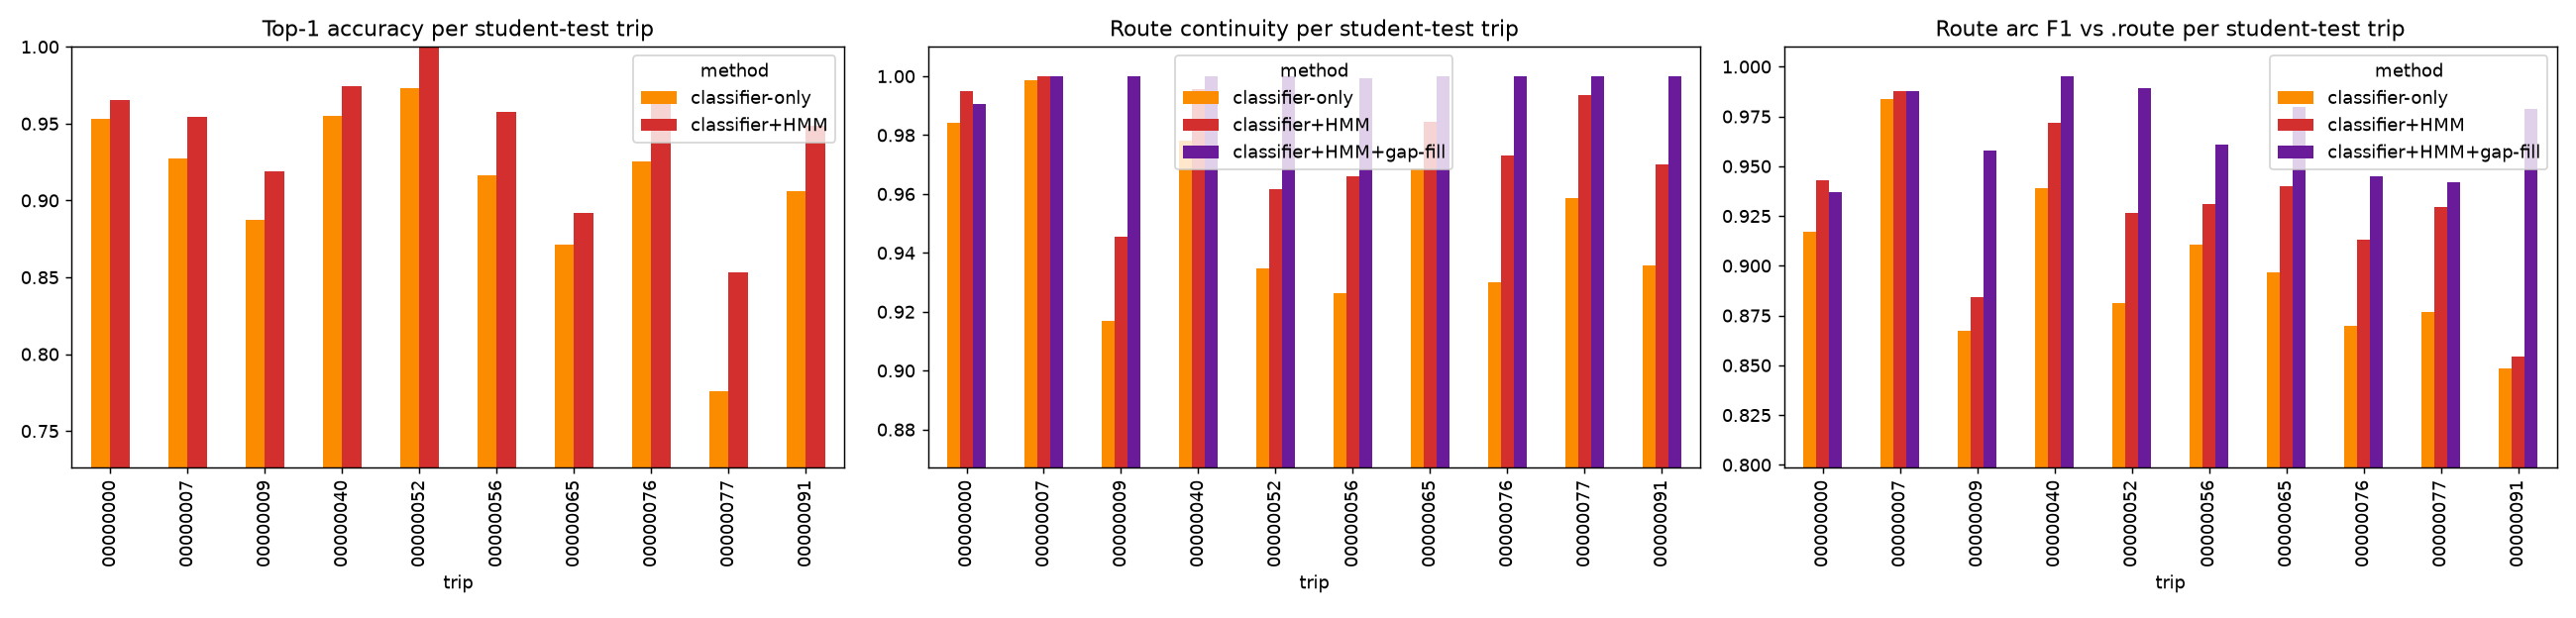
\includegraphics[width=\linewidth]{figures/hmm_per_trip.png}
  \caption{Per-trip Top-1, continuity and route F1: classifier only vs.\ HMM vs.\ HMM + gap filling.}
  \label{fig:hmmtrip}
\end{subfigure}\hfill
\begin{subfigure}{0.34\textwidth}
  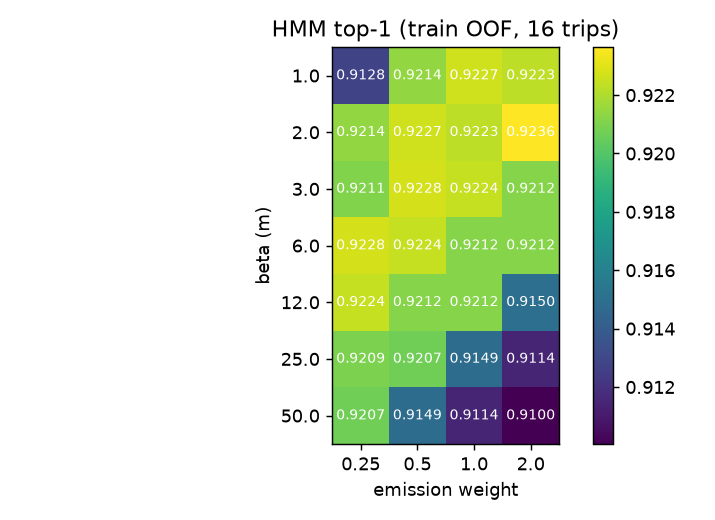
\includegraphics[width=\linewidth]{figures/hmm_grid.png}
  \caption{Decoder grid search on training trips (out-of-fold probabilities).}
\end{subfigure}
\caption{HMM results.}
\end{figure}

% =================================================================== 6
\section{Maps with Folium}

\code{scripts/05\_hmm.py} draws the trip maps and \code{scripts/01\_eda.py} draws the EDA maps, both from
the real pipeline output. The interactive HTML files are in \code{results/maps/} and \code{results/eda/}.
Every map shows:
\begin{itemize}
  \item the raw GPS readings (blue circles, with the timestamp on hover);
  \item the road network near the track (thin grey);
  \item the reference route (thick green);
  \item the classifier-only prediction (orange, hidden by default);
  \item the route rebuilt by the HMM (red);
  \item a legend with both Top-1 scores, and a control to switch layers on and off.
\end{itemize}
Each map zooms to fit its trip automatically.

\begin{figure}[H]
\centering
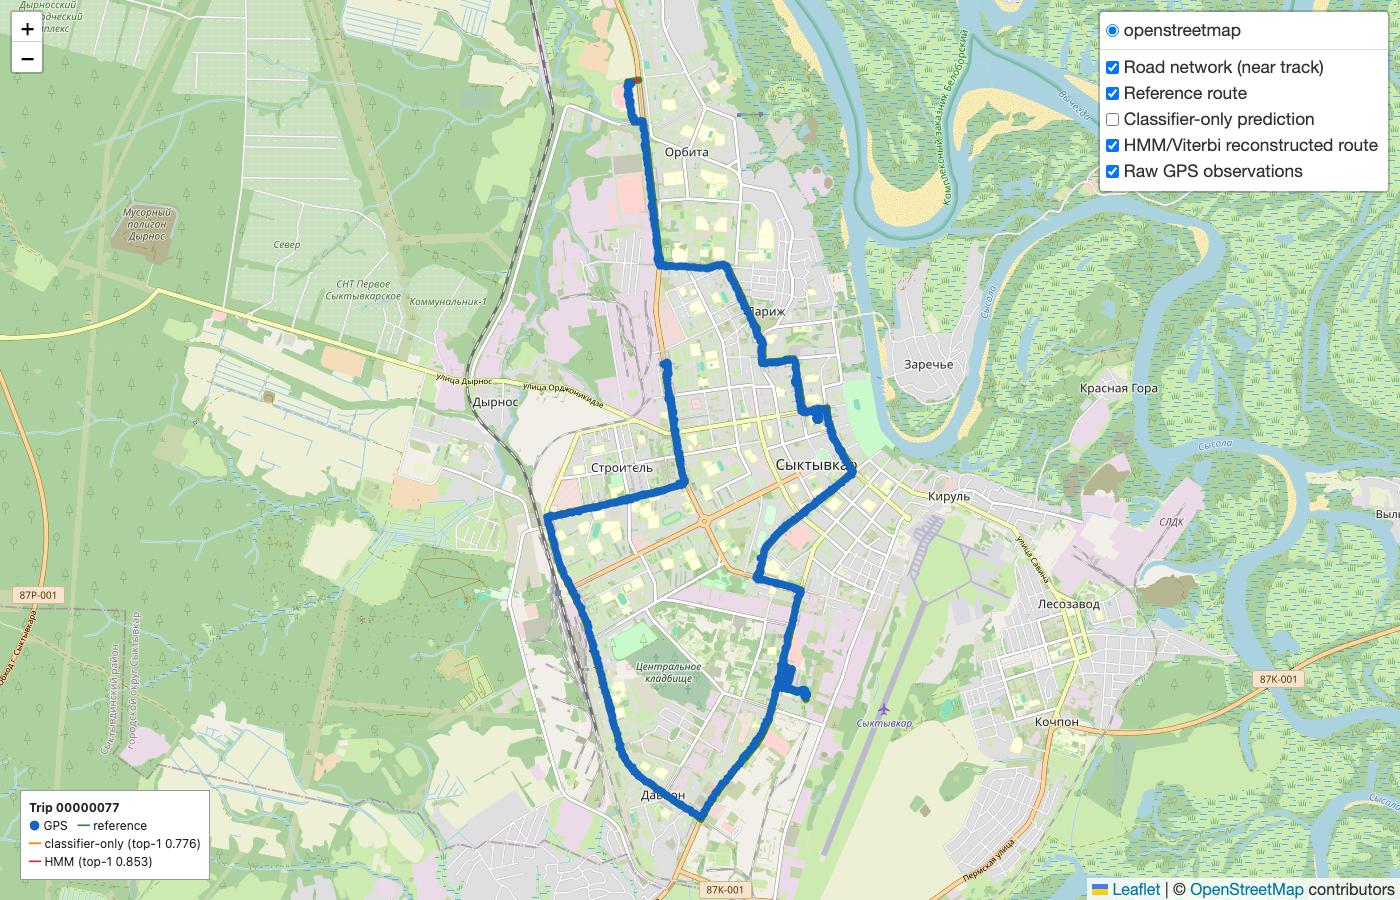
\includegraphics[width=0.85\textwidth]{figures/map_st77.png}
\caption{Student-test trip 00000077, our hardest trip: GPS (blue), reference route (green), HMM route (red)
and network (grey). Interactive version: \code{results/maps/student\_test\_00000077.html}.}
\end{figure}

\begin{figure}[H]
\centering
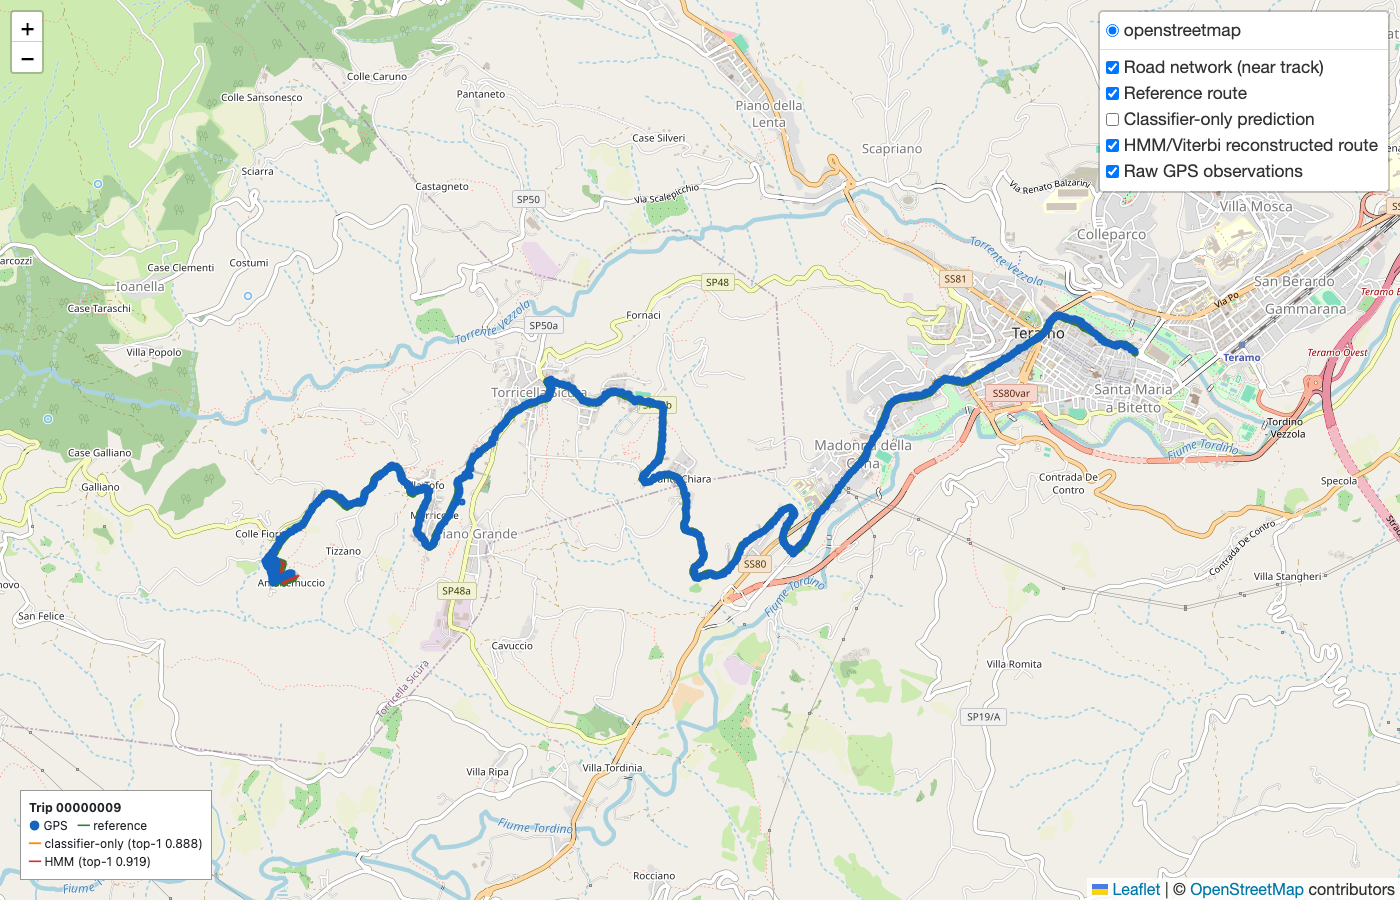
\includegraphics[width=0.85\textwidth]{figures/map_st09.png}
\caption{Student-test trip 00000009 with the layer control and legend (classifier-only Top-1 0.888, HMM
0.919). Interactive version: \code{results/maps/student\_test\_00000009.html}.}
\end{figure}

% =================================================================== 7
\section{API, UI and Deployment}

\paragraph{Laptop 1 -- the FastAPI server}
(\code{api/main.py}, started with \code{uvicorn api.main:app --host 0.0.0.0 --port 8000}).
\begin{itemize}
  \item When it starts, it loads \code{models/final\_model.joblib} and \code{configs/hmm\_config.json}.
  \item \code{GET /health} reports the model, the decoder settings and where the trips are coming from.
  \item \code{GET /trips} returns the trip ids and nothing else.
  \item \code{GET /models} lists every model you can pick: the deployed tuned XGBoost plus the seven models
        from Section~3 (retrained by \code{scripts/08\_export\_model\_zoo.py}), each with its offline CV and
        student-test scores.
  \item \code{POST /predict \{"trip\_id", "model"?, "use\_hmm"?\}} runs the whole pipeline. By default it uses
        the tuned XGBoost with the HMM switched on.
        \code{POST /compare \{"trip\_id"\}} runs every model on one trip, computing the features only once,
        and ranks them. All models share the HMM settings that were tuned for XGBoost.
  \item The pipeline always runs in this order: load $\rightarrow$ candidates $\rightarrow$ features
        $\rightarrow$ XGBoost $\rightarrow$ Viterbi $\rightarrow$ gap filling. Only after that does the
        server read the reference route to work out the accuracy.
  \item The response holds the GPS points, the predicted route lines, the metrics and the timings. The
        reference route itself is never sent.
  \item \textbf{Safety:} trip ids are checked against the folder listing, which also blocks path traversal.
  \item \textbf{Logs:} every request is logged (\code{PREDICT \ldots} / \code{RESULT \ldots}).
  \item \textbf{Nothing hard-coded:} the evaluator folder comes in through \code{PATHSNAP\_EVAL\_DIR}, and no
        code depends on any particular trip.
\end{itemize}

\paragraph{Laptop 2 -- the evaluator UI}
(\code{ui/index.html}, served with \code{python -m http.server 8501}).
This is a single Leaflet page. It lists the trips it gets from the API. When you click a trip, it sends the
id to \code{/predict}, draws the GPS points and the predicted route, and shows the metrics the server
computed. Under the metrics, an ``all models'' panel calls \code{POST /compare} and ranks every model on the
chosen trip by Top-1 with the HMM, alongside route F1 (Fig.~\ref{fig:uieval}). Each student-test trip takes
0.05--0.62\,s to process (median about 0.27\,s).

\subsection{Evaluation day (10 evaluator trips)}
\label{sec:evalday}

We ran the evaluator trips through the deployed pipeline exactly as it was (tuned XGBoost + HMM + gap
filling), using \code{POST /predict}. Nothing was retrained or re-tuned afterwards.
\begin{itemize}
  \item All 10 trips were processed, in 0.09--0.79\,s each.
  \item Top-1 accuracy went from 91.8\% with the classifier alone to 95.1\% with the HMM (mean over trips).
        Pooled over all 19,673 labelled points, it went from 86.5\% to 94.3\%.
  \item Mean route F1 was 93.6\%, and route continuity was 100\% on every trip.
  \item The HMM improved every trip. The biggest jump was trip 00000015, from 70.5\% to 90.2\%.
  \item Route precision was lowest on trips 00000015 and 00000023 (65\%, with recall above 98\%). This is
        the known cost of shortest-path gap filling (Section~\ref{sec:hmm}).
\end{itemize}

\begin{table}[H]
\centering
\small
\begin{tabular}{@{}lrccc@{}}
\toprule
\textbf{Trip} & \textbf{Points} & \textbf{Top-1 classifier} & \textbf{Top-1 HMM} & \textbf{Route F1} \\
\midrule
00000015 & 6,854 & 0.7049 & 0.9022 & 0.7836 \\
00000017 & 1,346 & 0.9361 & 0.9458 & 0.9367 \\
00000023 & 458 & 0.9432 & 0.9541 & 0.7785 \\
00000030 & 654 & 0.8073 & 0.8364 & 0.9442 \\
00000049 & 2,642 & 0.9928 & 1.0000 & 0.9988 \\
00000059 & 1,031 & 0.9699 & 0.9777 & 0.9559 \\
00000067 & 916 & 0.9509 & 0.9596 & 0.9878 \\
00000073 & 1,144 & 0.9825 & 0.9851 & 0.9937 \\
00000087 & 1,399 & 0.9557 & 0.9964 & 0.9989 \\
00000094 & 3,230 & 0.9325 & 0.9492 & 0.9805 \\
\bottomrule
\end{tabular}
\caption{Evaluator-trip results. Source: \code{scripts/09\_evaluator\_run.py} $\rightarrow$
\code{results/evaluator/evaluator\_results.csv} and \code{summary.json}. The script runs the same deployed
pipeline as the API, and the interactive maps are in \code{results/maps/evaluator\_*.html}.}
\end{table}

\begin{figure}[H]
\centering
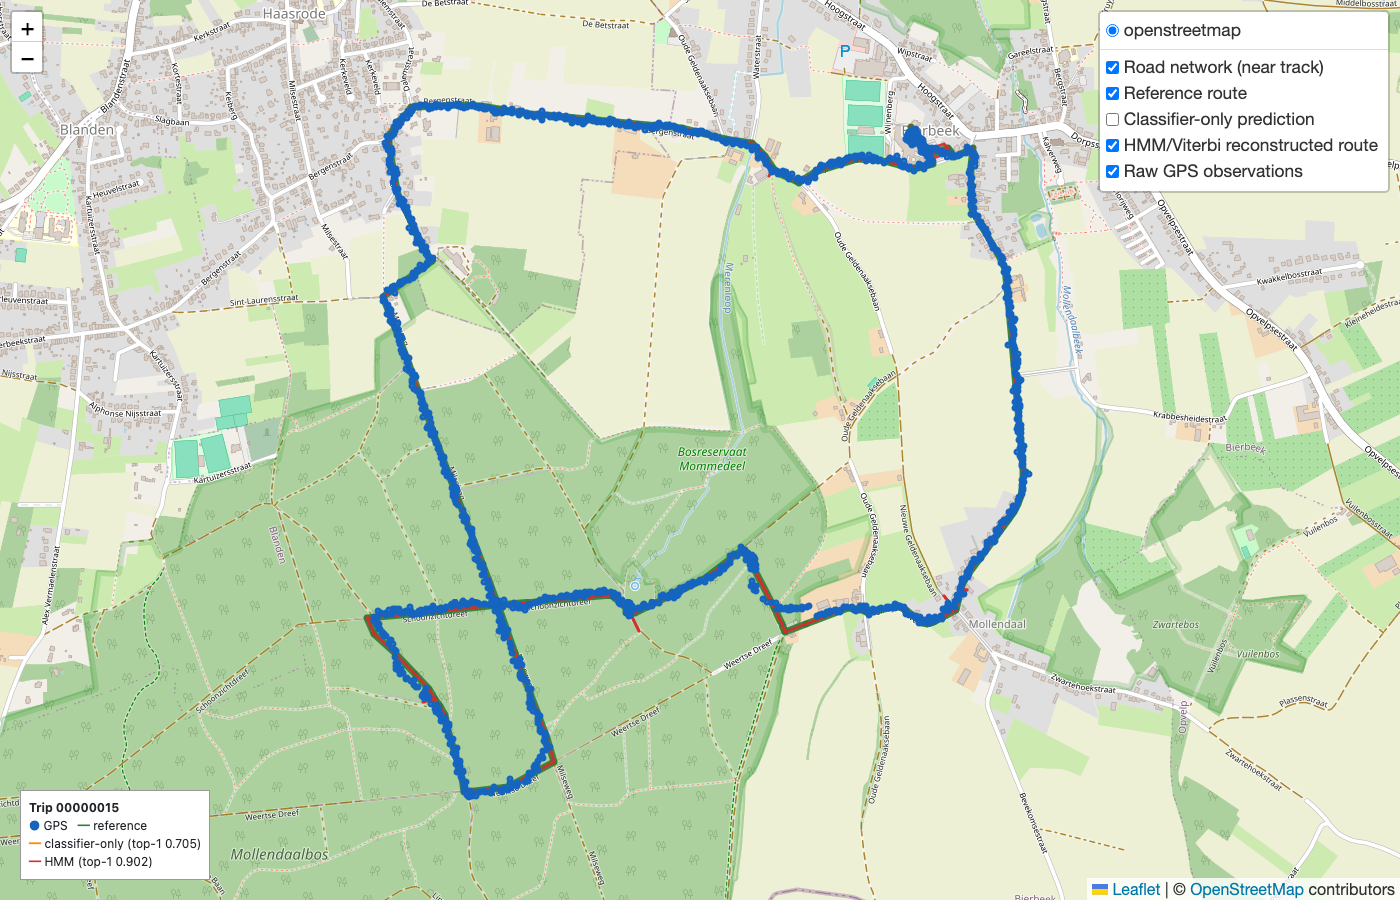
\includegraphics[width=0.85\textwidth]{figures/map_eval15.png}
\caption{Evaluator trip 00000015 (Folium): GPS (blue), reference route (green) and the HMM route (red). The
legend shows classifier-only Top-1 0.705 vs.\ HMM 0.902.}
\end{figure}

\begin{figure}[H]
\centering
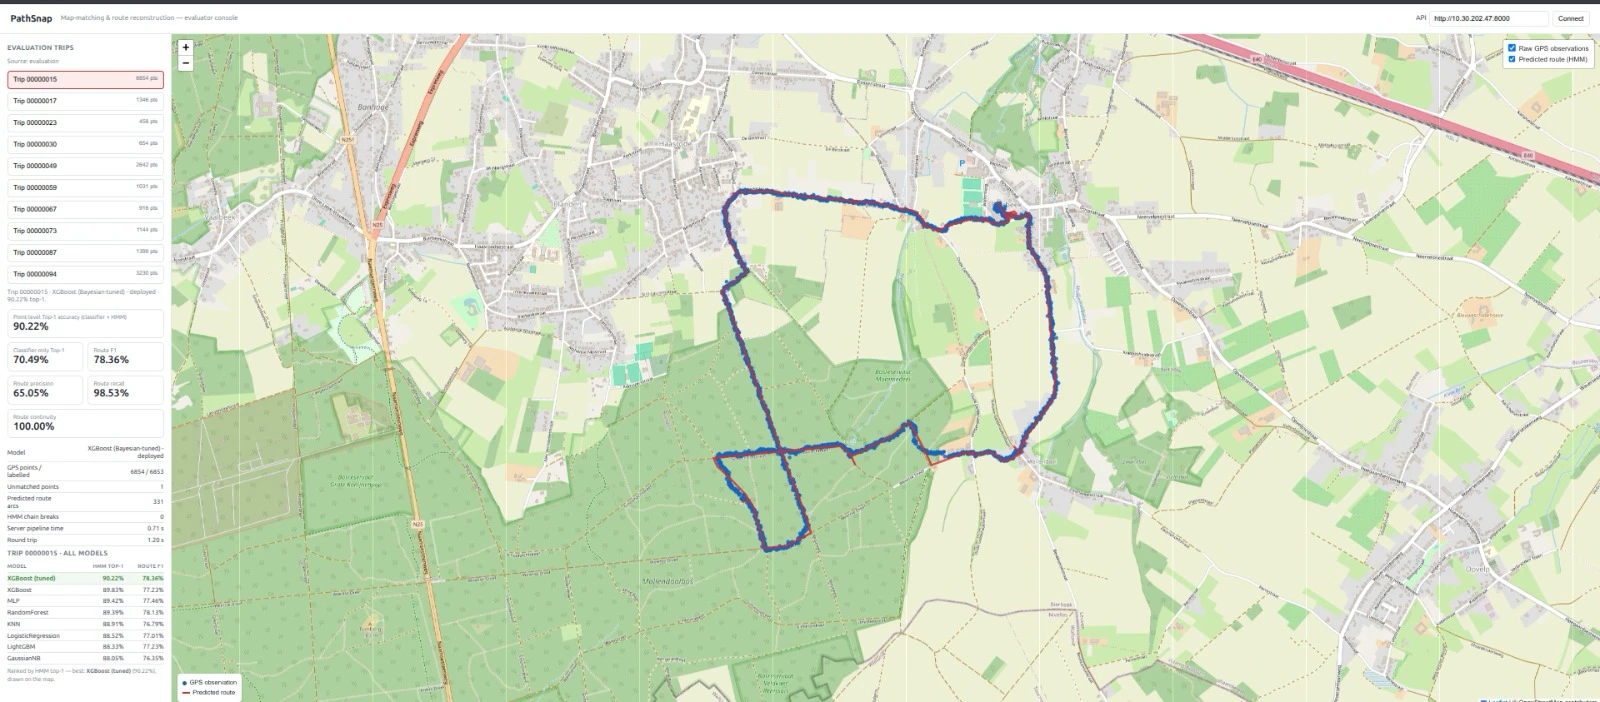
\includegraphics[width=\textwidth]{figures/ui_eval.png}
\caption{The evaluator UI on Laptop~2, connected to the API on Laptop~1 (\code{http://10.30.202.47:8000}).
Evaluator trip 00000015 is selected: GPS points (blue) and the HMM route (red), Top-1 90.22\% with the HMM
vs.\ 70.49\% for the classifier alone, route F1 78.36\%, continuity 100\%. The panel under the metrics ranks
every model on this trip using \code{POST /compare}.}
\label{fig:uieval}
\end{figure}

\begin{figure}[H]
\centering
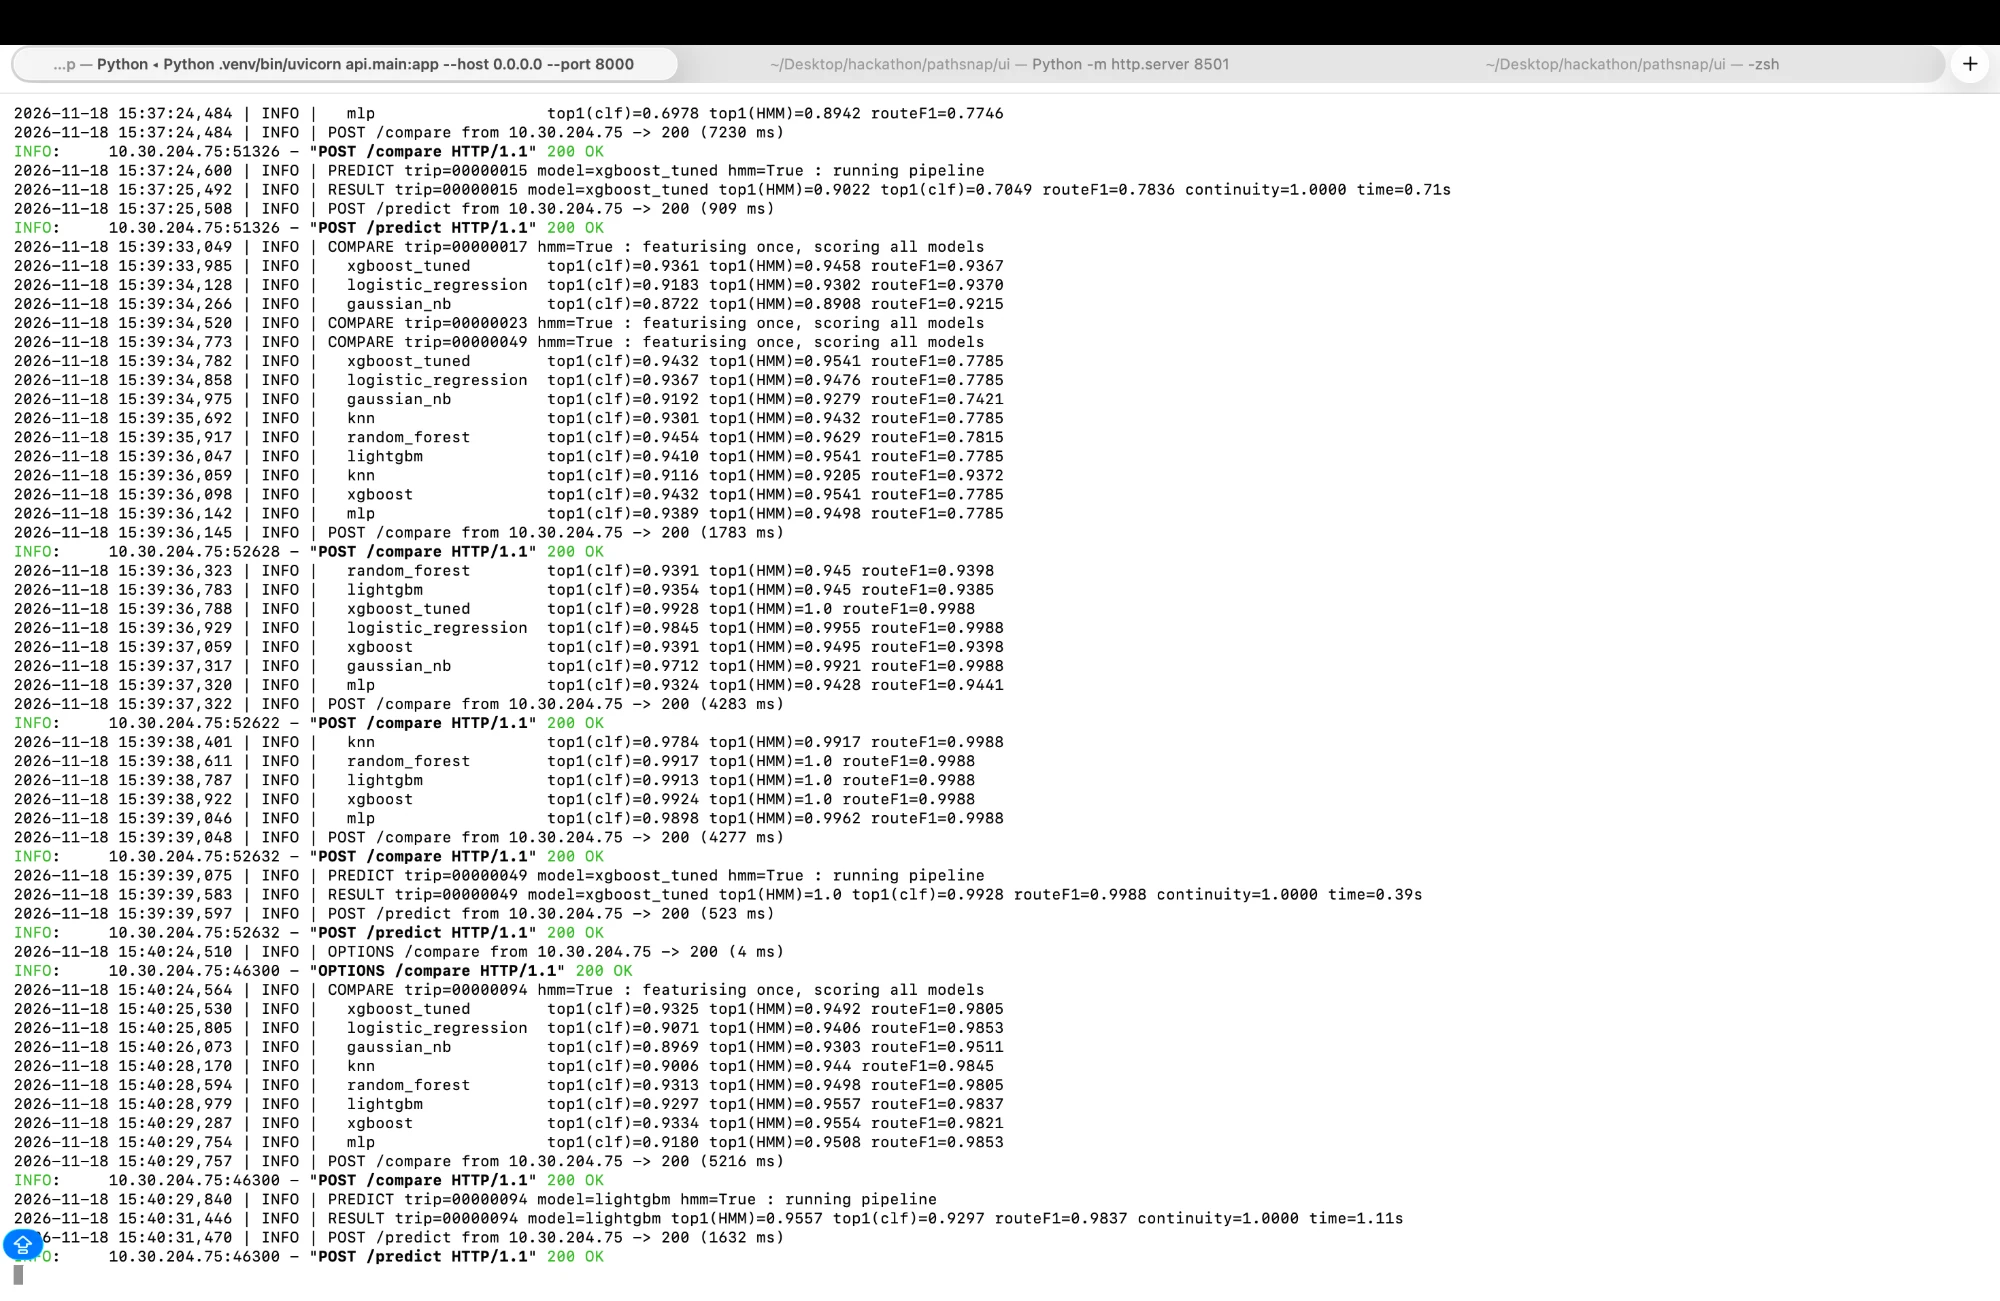
\includegraphics[width=\textwidth]{figures/api_logs.png}
\caption{API logs on Laptop~1. Every request comes from Laptop~2 (10.30.204.75) and returns 200. The
\code{COMPARE} lines score all models on trips 00000017, 00000023, 00000049 and 00000094. The
\code{PREDICT}/\code{RESULT} lines show trip 00000015 with the deployed model (Top-1 0.9022 with the HMM,
0.7049 without), trip 00000049 (1.0), and trip 00000094 with LightGBM selected (0.9557).}
\end{figure}

\begin{figure}[H]
\centering
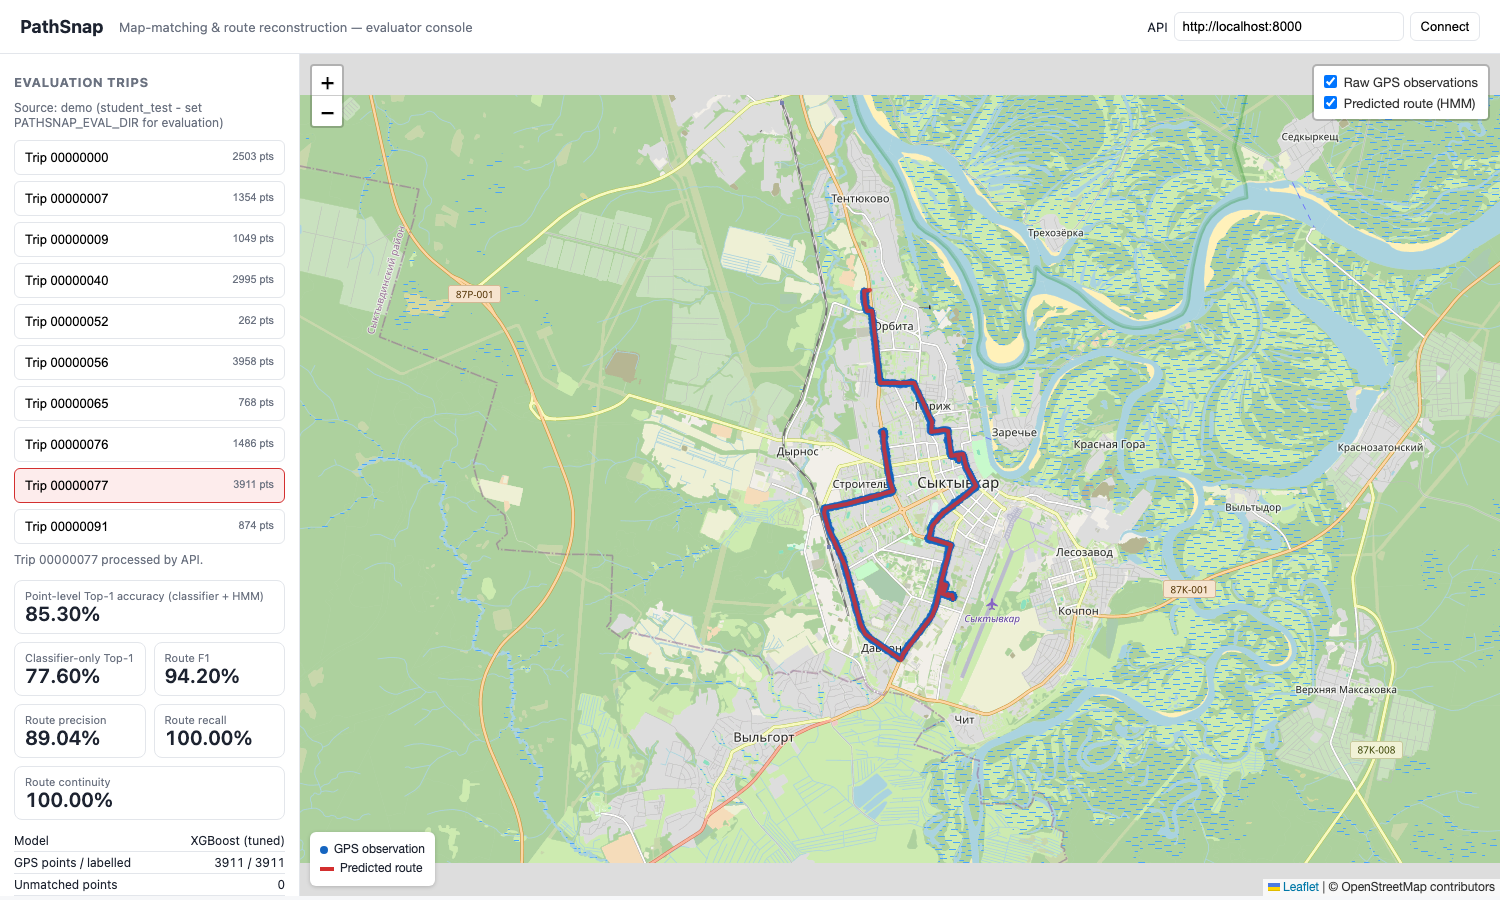
\includegraphics[width=0.85\textwidth]{figures/ui_dev77.png}
\caption{The UI during development (student-test trip 00000077): the trip list, the metrics computed on the
server (Top-1 with HMM 85.30\%, classifier only 77.60\%, route F1 94.20\%, continuity 100\%), and the
predicted route over OpenStreetMap.}
\end{figure}

% =================================================================== 8
\section{Integrity, Limitations and Use of AI}

\subsection{How we avoided leakage}
\begin{itemize}
  \item We did not have the evaluator data during development. We got it on evaluation day and used it only
        to run the deployed API (Section~\ref{sec:evalday}). Nothing was retrained or re-tuned on it.
  \item All fitting, cross-validation and Bayesian optimisation used training trips only, with folds grouped
        by trip.
  \item The StandardScalers (for LR, KNN and MLP) sit inside the pipelines, so they are fitted on the
        training folds only.
  \item The decoder settings were tuned on out-of-fold training predictions.
  \item We used student-test results only to compare approaches during development, never to pick the
        deployed hyperparameters.
  \item The predictor reads only \code{.track}, \code{.nodes} and \code{.arcs}. The \code{.route} file is
        read only by the evaluation function, after the prediction is made.
\end{itemize}

\subsection{Limitations}
\begin{itemize}
  \item The point-level labels come from aligning points to \code{.route}. Near junctions it is unclear
        where one arc ends and the next begins, so some of the remaining error is label noise rather than
        model error.
  \item The reference routes are not perfect either. We had to drop two training trips where the GPS and
        the route disagree (Section~2.1).
  \item The transition model ignores turn angles and road types. Gap filling uses shortest paths, which
        costs a little route precision.
  \item Results on new trips may differ from student-test. The trips come from many different cities, and
        10 trips is a small sample.
\end{itemize}

\subsection{Use of AI assistance}
As the event's policy requires, we are disclosing that we built this project with a lot of help from an AI
coding assistant: Anthropic's Claude, used through the Claude Code desktop app.

\textbf{What the assistant did.} It wrote most of the source code: data loading, projection, label
alignment, candidate generation and features, the seven training pipelines, the Bayesian optimisation, the
HMM/Viterbi decoder, the FastAPI server and the UI. It ran the scripts on our laptop, and it drafted this
report and our viva notes from the outputs of those runs.

\textbf{What we did.} We read the hackathon documents and set the task, supplied and organised the dataset,
asked for each part and then reviewed and tested it, set up GitHub and the two-laptop deployment, ran the
evaluation-day demo, took the deployment screenshots, and reviewed and edited this report.

\textbf{Results are real.} Every metric, table and figure here was produced by running the code in the
repository. None of it was typed in by hand, and every figure can be regenerated with the scripts in
Section~\ref{sec:repro}.

\textbf{We understand it.} Every team member has gone through the code, the experiments and this report,
and can explain the design decisions, the models and the results.

\subsection{Reproducing our results}
\label{sec:repro}
\begin{verbatim}
pip install -r requirements.txt        # macOS: brew install libomp
python scripts/01_eda.py
python scripts/02_build_features.py
python scripts/03_train_models.py
python scripts/04_bayes_opt.py 30
python scripts/05_hmm.py
python scripts/06_collect_results.py
python scripts/07_report_assets.py
python scripts/08_export_model_zoo.py
python scripts/09_evaluator_run.py     # evaluation day only
\end{verbatim}

\end{document}
